
%% bare_conf.tex
%% V1.4b
%% 2015/08/26
%% by Michael Shell
%% See:
%% http://www.michaelshell.org/
%% for current contact information.
%%
%% This is a skeleton file demonstrating the use of IEEEtran.cls
%% (requires IEEEtran.cls version 1.8b or later) with an IEEE
%% conference paper.
%%
%% Support sites:
%% http://www.michaelshell.org/tex/ieeetran/
%% http://www.ctan.org/pkg/ieeetran
%% and
%% http://www.ieee.org/

%%*************************************************************************
%% Legal Notice:
%% This code is offered as-is without any warranty either expressed or
%% implied; without even the implied warranty of MERCHANTABILITY or
%% FITNESS FOR A PARTICULAR PURPOSE! 
%% User assumes all risk.
%% In no event shall the IEEE or any contributor to this code be liable for
%% any damages or losses, including, but not limited to, incidental,
%% consequential, or any other damages, resulting from the use or misuse
%% of any information contained here.
%%
%% All comments are the opinions of their respective authors and are not
%% necessarily endorsed by the IEEE.
%%
%% This work is distributed under the LaTeX Project Public License (LPPL)
%% ( http://www.latex-project.org/ ) version 1.3, and may be freely used,
%% distributed and modified. A copy of the LPPL, version 1.3, is included
%% in the base LaTeX documentation of all distributions of LaTeX released
%% 2003/12/01 or later.
%% Retain all contribution notices and credits.
%% ** Modified files should be clearly indicated as such, including  **
%% ** renaming them and changing author support contact information. **
%%*************************************************************************


% *** Authors should verify (and, if needed, correct) their LaTeX system  ***
% *** with the testflow diagnostic prior to trusting their LaTeX platform ***
% *** with production work. The IEEE's font choices and paper sizes can   ***
% *** trigger bugs that do not appear when using other class files.       ***                          ***
% The testflow support page is at:
% http://www.michaelshell.org/tex/testflow/



\documentclass[conference]{IEEEtran}
% Some Computer Society conferences also require the compsoc mode option,
% but others use the standard conference format.
%
% If IEEEtran.cls has not been installed into the LaTeX system files,
% manually specify the path to it like:
% \documentclass[conference]{../sty/IEEEtran}





% Some very useful LaTeX packages include:
% (uncomment the ones you want to load)


% *** MISC UTILITY PACKAGES ***
%
%\usepackage{ifpdf}
% Heiko Oberdiek's ifpdf.sty is very useful if you need conditional
% compilation based on whether the output is pdf or dvi.
% usage:
% \ifpdf
%   % pdf code
% \else
%   % dvi code
% \fi
% The latest version of ifpdf.sty can be obtained from:
% http://www.ctan.org/pkg/ifpdf
% Also, note that IEEEtran.cls V1.7 and later provides a builtin
% \ifCLASSINFOpdf conditional that works the same way.
% When switching from latex to pdflatex and vice-versa, the compiler may
% have to be run twice to clear warning/error messages.






% *** CITATION PACKAGES ***
%
\usepackage{cite}
% cite.sty was written by Donald Arseneau
% V1.6 and later of IEEEtran pre-defines the format of the cite.sty package
% \cite{} output to follow that of the IEEE. Loading the cite package will
% result in citation numbers being automatically sorted and properly
% "compressed/ranged". e.g., [1], [9], [2], [7], [5], [6] without using
% cite.sty will become [1], [2], [5]--[7], [9] using cite.sty. cite.sty's
% \cite will automatically add leading space, if needed. Use cite.sty's
% noadjust option (cite.sty V3.8 and later) if you want to turn this off
% such as if a citation ever needs to be enclosed in parenthesis.
% cite.sty is already installed on most LaTeX systems. Be sure and use
% version 5.0 (2009-03-20) and later if using hyperref.sty.
% The latest version can be obtained at:
% http://www.ctan.org/pkg/cite
% The documentation is contained in the cite.sty file itself.






% *** GRAPHICS RELATED PACKAGES ***
%
\ifCLASSINFOpdf
   \usepackage[pdftex]{graphicx}
  % declare the path(s) where your graphic files are
  % \graphicspath{{../pdf/}{../jpeg/}}
  % and their extensions so you won't have to specify these with
  % every instance of \includegraphics
   \DeclareGraphicsExtensions{.pdf,.jpeg,.png}
\else
  % or other class option (dvipsone, dvipdf, if not using dvips). graphicx
  % will default to the driver specified in the system graphics.cfg if no
  % driver is specified.
  % \usepackage[dvips]{graphicx}
  % declare the path(s) where your graphic files are
  % \graphicspath{{../eps/}}
  % and their extensions so you won't have to specify these with
  % every instance of \includegraphics
  % \DeclareGraphicsExtensions{.eps}
\fi
% graphicx was written by David Carlisle and Sebastian Rahtz. It is
% required if you want graphics, photos, etc. graphicx.sty is already
% installed on most LaTeX systems. The latest version and documentation
% can be obtained at: 
% http://www.ctan.org/pkg/graphicx
% Another good source of documentation is "Using Imported Graphics in
% LaTeX2e" by Keith Reckdahl which can be found at:
% http://www.ctan.org/pkg/epslatex
%
% latex, and pdflatex in dvi mode, support graphics in encapsulated
% postscript (.eps) format. pdflatex in pdf mode supports graphics
% in .pdf, .jpeg, .png and .mps (metapost) formats. Users should ensure
% that all non-photo figures use a vector format (.eps, .pdf, .mps) and
% not a bitmapped formats (.jpeg, .png). The IEEE frowns on bitmapped formats
% which can result in "jaggedy"/blurry rendering of lines and letters as
% well as large increases in file sizes.
%
% You can find documentation about the pdfTeX application at:
% http://www.tug.org/applications/pdftex





% *** MATH PACKAGES ***
%
%\usepackage{amsmath}
% A popular package from the American Mathematical Society that provides
% many useful and powerful commands for dealing with mathematics.
%
% Note that the amsmath package sets \interdisplaylinepenalty to 10000
% thus preventing page breaks from occurring within multiline equations. Use:
%\interdisplaylinepenalty=2500
% after loading amsmath to restore such page breaks as IEEEtran.cls normally
% does. amsmath.sty is already installed on most LaTeX systems. The latest
% version and documentation can be obtained at:
% http://www.ctan.org/pkg/amsmath





% *** SPECIALIZED LIST PACKAGES ***
%
%\usepackage{algorithmic}
% algorithmic.sty was written by Peter Williams and Rogerio Brito.
% This package provides an algorithmic environment fo describing algorithms.
% You can use the algorithmic environment in-text or within a figure
% environment to provide for a floating algorithm. Do NOT use the algorithm
% floating environment provided by algorithm.sty (by the same authors) or
% algorithm2e.sty (by Christophe Fiorio) as the IEEE does not use dedicated
% algorithm float types and packages that provide these will not provide
% correct IEEE style captions. The latest version and documentation of
% algorithmic.sty can be obtained at:
% http://www.ctan.org/pkg/algorithms
% Also of interest may be the (relatively newer and more customizable)
% algorithmicx.sty package by Szasz Janos:
% http://www.ctan.org/pkg/algorithmicx




% *** ALIGNMENT PACKAGES ***
%
%\usepackage{array}
% Frank Mittelbach's and David Carlisle's array.sty patches and improves
% the standard LaTeX2e array and tabular environments to provide better
% appearance and additional user controls. As the default LaTeX2e table
% generation code is lacking to the point of almost being broken with
% respect to the quality of the end results, all users are strongly
% advised to use an enhanced (at the very least that provided by array.sty)
% set of table tools. array.sty is already installed on most systems. The
% latest version and documentation can be obtained at:
% http://www.ctan.org/pkg/array


% IEEEtran contains the IEEEeqnarray family of commands that can be used to
% generate multiline equations as well as matrices, tables, etc., of high
% quality.




% *** SUBFIGURE PACKAGES ***
%\ifCLASSOPTIONcompsoc
%  \usepackage[caption=false,font=normalsize,labelfont=sf,textfont=sf]{subfig}
%\else
%  \usepackage[caption=false,font=footnotesize]{subfig}
%\fi
% subfig.sty, written by Steven Douglas Cochran, is the modern replacement
% for subfigure.sty, the latter of which is no longer maintained and is
% incompatible with some LaTeX packages including fixltx2e. However,
% subfig.sty requires and automatically loads Axel Sommerfeldt's caption.sty
% which will override IEEEtran.cls' handling of captions and this will result
% in non-IEEE style figure/table captions. To prevent this problem, be sure
% and invoke subfig.sty's "caption=false" package option (available since
% subfig.sty version 1.3, 2005/06/28) as this is will preserve IEEEtran.cls
% handling of captions.
% Note that the Computer Society format requires a larger sans serif font
% than the serif footnote size font used in traditional IEEE formatting
% and thus the need to invoke different subfig.sty package options depending
% on whether compsoc mode has been enabled.
%
% The latest version and documentation of subfig.sty can be obtained at:
% http://www.ctan.org/pkg/subfig




% *** FLOAT PACKAGES ***
%
%\usepackage{fixltx2e}
% fixltx2e, the successor to the earlier fix2col.sty, was written by
% Frank Mittelbach and David Carlisle. This package corrects a few problems
% in the LaTeX2e kernel, the most notable of which is that in current
% LaTeX2e releases, the ordering of single and double column floats is not
% guaranteed to be preserved. Thus, an unpatched LaTeX2e can allow a
% single column figure to be placed prior to an earlier double column
% figure.
% Be aware that LaTeX2e kernels dated 2015 and later have fixltx2e.sty's
% corrections already built into the system in which case a warning will
% be issued if an attempt is made to load fixltx2e.sty as it is no longer
% needed.
% The latest version and documentation can be found at:
% http://www.ctan.org/pkg/fixltx2e


%\usepackage{stfloats}
% stfloats.sty was written by Sigitas Tolusis. This package gives LaTeX2e
% the ability to do double column floats at the bottom of the page as well
% as the top. (e.g., "\begin{figure*}[!b]" is not normally possible in
% LaTeX2e). It also provides a command:
%\fnbelowfloat
% to enable the placement of footnotes below bottom floats (the standard
% LaTeX2e kernel puts them above bottom floats). This is an invasive package
% which rewrites many portions of the LaTeX2e float routines. It may not work
% with other packages that modify the LaTeX2e float routines. The latest
% version and documentation can be obtained at:
% http://www.ctan.org/pkg/stfloats
% Do not use the stfloats baselinefloat ability as the IEEE does not allow
% \baselineskip to stretch. Authors submitting work to the IEEE should note
% that the IEEE rarely uses double column equations and that authors should try
% to avoid such use. Do not be tempted to use the cuted.sty or midfloat.sty
% packages (also by Sigitas Tolusis) as the IEEE does not format its papers in
% such ways.
% Do not attempt to use stfloats with fixltx2e as they are incompatible.
% Instead, use Morten Hogholm'a dblfloatfix which combines the features
% of both fixltx2e and stfloats:
%
% \usepackage{dblfloatfix}
% The latest version can be found at:
% http://www.ctan.org/pkg/dblfloatfix

\usepackage{subfig}

% *** PDF, URL AND HYPERLINK PACKAGES ***
%
\usepackage{url}
% url.sty was written by Donald Arseneau. It provides better support for
% handling and breaking URLs. url.sty is already installed on most LaTeX
% systems. The latest version and documentation can be obtained at:
% http://www.ctan.org/pkg/url
% Basically, \url{my_url_here}.


\usepackage{color,soul}
\usepackage{xspace}
\newcommand{\TODO}[1]{\hl{\textbf{TODO:} #1}\xspace}
\newcommand{\todo}[1]{\TODO{#1}}

% \newfont{\nicettfont}{cmtt9}
% \newcommand{\ndnName}[1]{``{\nicettfont \url{#1}}''}
% \newcommand{\ndnNameUnquoted}[1]{{\nicettfont \url{#1}}}

%% \ndnName command
%% - allows break before /
\usepackage{etoolbox}
\usepackage{xstring}
\DeclareListParser{\doslashlist}{/}
\newcounter{ndnNameComponentCounter}%
\newcommand{\ndnName}[1]{{%
  \setcounter{ndnNameComponentCounter}{0}%
  \renewcommand{\do}[1]{{%
    \ifnumgreater{\value{ndnNameComponentCounter}}{0}{\allowbreak/}{}%
    \ifnumodd{\value{ndnNameComponentCounter}}{}{}%
    \detokenize{##1}}%
    \stepcounter{ndnNameComponentCounter}}%
``{\fontfamily{cmtt}\small\selectfont\IfBeginWith{#1}{/}{/}{}\doslashlist{#1}}''%
}}

% *** Do not adjust lengths that control margins, column widths, etc. ***
% *** Do not use packages that alter fonts (such as pslatex).         ***
% There should be no need to do such things with IEEEtran.cls V1.6 and later.
% (Unless specifically asked to do so by the journal or conference you plan
% to submit to, of course. )


% correct bad hyphenation here
\hyphenation{op-tical net-works semi-conduc-tor}

\graphicspath{{figures/}}

\begin{document}

%\title{A Cloud-Independent Home Entertainment Design over Named Data Networking of Things}

\title{Named Data Networking of Things and Example Application ``Flow''}

% for over three affiliations, or if they all won't fit within the width
% of the page, use this alternative format:
% 
\author{\IEEEauthorblockN{
Zhehao Wang, 
% \IEEEauthorrefmark{2}
% \IEEEauthorrefmark{1},
Jeff Burke
% \IEEEauthorrefmark{2}
% \IEEEauthorblockA{\IEEEauthorrefmark{1}UCLA Internet Research Laboratory,
% \{zhehao\}@cs.ucla.edu}
% \IEEEauthorblockA{\IEEEauthorrefmark{2}UCLA Center for Research in Engineering, Media and Performance,
% \{zhehao,jburke\}@remap.ucla.edu}}}
}}

% use for special paper notices

% make the title area
\maketitle

% As a general rule, do not put math, special symbols or citations
% in the abstract
\begin{abstract}
    %% abstract
In this report we introduce the application Flow, a prototype home entertainment experience built using Named Data Networking (NDN). Flow provides an exploratory experience in which a player navigates and interacts with a virtual environment via person tracking (OpenPTrack), wearable devices (gyroscope), and their mobile phone. 
Through this application we showed an approach to achieve two fundamental functions in IoT, trust management and rendezvous, in a way that does not rely on (but can incorporate) cloud-based services.
At the heart of the design are application-defined hierarchically named and secured data packets exchanged at the networking level, from which trust management and rendezvous can be built. 
To develop Flow, we designed and implemented the Named Data Networking of Things (NDN-IoT) framework, libraries in multiple languages that implement naming, trust and bootstrap, discovery, and application level pub/sub, to explore IoT-based application development in a home environment.
While a high-level design of the framework and application can be found in the author's IOTDI 2017 invited paper, this report focuses on low-level details, including library workflow and interfaces, with in-application examples.

% Many emerging IoT approaches depend on cloud services to facilitate interoperation of devices and services within them, even when the primary need for communication is local in scope, as in many ``smart home'' applictions.
% While such designs offer a convenient way to implement IoT applications using today's TCP/IP Internet architecture, they also introduce dependencies between  applications and Internet connectivity that are unnecessary and often brittle.
% % danger for users to lose access to their homes if the Internet goes down. 
% This paper uses the design of an IoT-enabled home entertainment experience to demonstrate how the Named Data Networking (NDN) architecture enables cloud-independent IoT applications.
% It does so by enabling local trust management and rendezvous, which play a foundational role in realizing other IoT services.  By employing application-defined naming rather than host-based addressing at the network layer, and securing data directly,
% NDN enables straightforward and robust implementation of these two core functions for IoT networks with or without cloud connectivity.
% %Further, the architecture's intrinsic support for ad hoc and potentially intermittent connectivity enables these functions to existing robustly among home IoT devices with or without cloud connectivity. 
% %NDN intrinsically supports local, ad hoc, and potentially intermittent connectivity, robustly enabling this functionality among home IoT devices.
% At the same time, 
% NDN-based IoT designs can also employ cloud services to complement local system capabilities.  After describing the motivation, design, and preliminary generalization of the driver application, the paper concludes with a brief comparison with how it would be achieved using two popular IoT frameworks, Amazon's AWS IoT service and the Apple HomeKit framework.
% %However, we believe it is critically important that home applications do not depend on cloud, to achieve resilient local operations independent from external failures.

\end{abstract}

% no keywords

%%% paper outline:
%%%  https://docs.google.com/document/d/1wo7QXH9EV1xWYPfviLX7_s23c1ZmtjW5N5C_VvuRxSA/edit?usp=sharing
%%%

% \section{Introduction}
\label{sec:introduction}

% Outline: IoT for home entertainment
Internet-of-Things (IoT) technologies are being rapidly adopted in the consumer electronics market.
In addition to their use in traditional home automation systems, IoT technologies have also been applied to home entertainment--for example, with wireless inertial sensors used to track user body movement in sports games. 
Combined with emerging virtual and augmented reality technologies, IoT offers the promise of new immersive and interactive experience for end-users.

Common requirements for such systems include:
\begin{itemize}
\item Integration of heterogeneous devices and services from different vendors;
\item Interactive user experience that emphasize real-time feedback loop;
\item Easy installation and configuration; and
\item Security protection, due to tight integration with the home network.
\end{itemize}

% Outline: existing frameworks and their functionality summary
Many IoT frameworks and ecosystems have been proposed over the last few years to facilitate the development of more sophisticated applications like these.
They typically provide a similar set of framework-level services, including user and device authentication and authorization, device and service discovery, device management, publish-subscribe messaging, and remote access.
Fig.~\ref{fig:service-arch} shows a common hierarchical architecture of IoT services, where ``named entities'' refer to users, devices, and applications that require trust management and utilize rendezvous services to get organized into a coherent home IoT system.

\begin{figure}[!t]
\centering
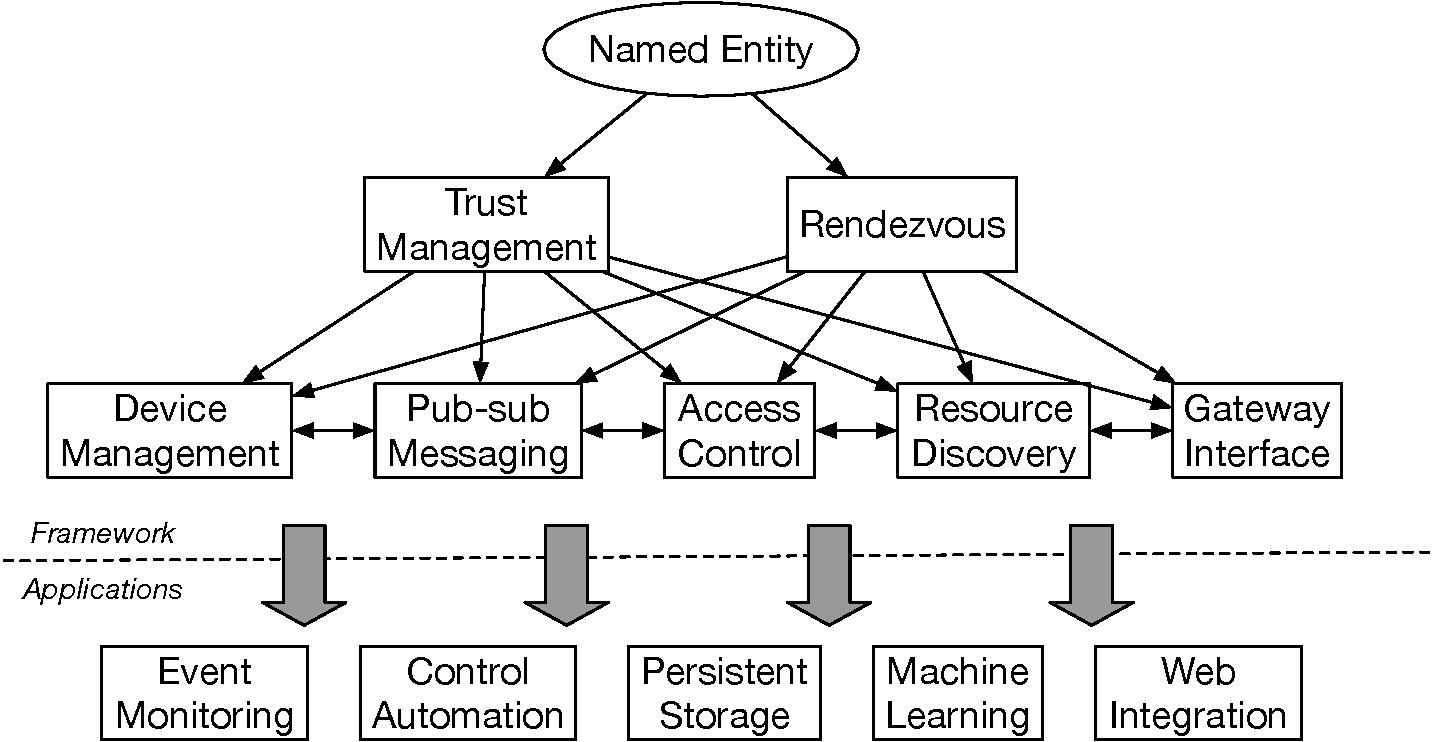
\includegraphics[width=0.95\columnwidth]{service-arch.pdf}
\caption{Hierarchical architecture of IoT services.}
\label{fig:service-arch}
\end{figure}

% Outline: introducing Flow
% Citation mark
The authors' cite:iotdi-2017 paper described an NDN approach~\cite{ccn-van,ndn}, which builds on our previous work in~\cite{ndn-iot} and focuses on foundational functions of \emph{trust management} and \emph{rendezvous}.
\footnote{For background study, conceptual comparison between our approach and existing ones, please refer to this paper as well.}
While in the same paper the authors used Flow, an IoT-augmented home entertainment experience, to illustrate the high-level concepts, this report describes the design and implementation of Flow and its supporting libraries in more detail.

% Outline: the rest of the paper
In Section~\ref{sec:flow-overview}, we first give an introduction of Flow application and its requirements. Generalizing from its requirements we also propose an NDN-IoT framework, a set of IoT libraries built to support applications like Flow. 
In Sections~\ref{sec:components} and~\ref{sec:implementation}, we present the design and implementation details of Flow. 
% TODO: what do we conclude with
We conclude with a.


% \section{Background}
\label{sec:background}

\subsection{Existing IoT Ecosystems}
\label{sec:iot-ecosystems}

Many current IoT architectures and frameworks, such as Bluetooth~\cite{bluetooth}, ZigBee~\cite{zigbee}, and Google Thread~\cite{thread}, have primarily focused on achieving device-to-device connectivity and interoperability.
For example, Bluetooth defines a seven-layer protocol stack and how two devices can connect to each other over either point-to-point or mesh networks, discover the other's capabilities through application layer profiles, and exchange application data called attributes.
Designed as silos, these architectures cannot interoperate with each other without special gateway or translator deployed in between, limiting development and innovation of IoT technologies.

% JB: How does preceding sentence and this paragraph relate to overall thesis of paper? 
As the IoT systems become more powerful and more complex, there is a growing demand for more comprehensive application-layer frameworks that can integrate and manage different types of devices across different communication technologies, enable more intelligent application logic involving a large number of devices, and provide simplified user experience in operating such systems.
In this subsection, we briefly review a few popular IoT application frameworks that appeared in the last three years.

\emph{AllJoyn}~(2013\footnote{The number in parentheses indicates the year of initial public announcement.})~\cite{alljoyn} and \emph{IoTivity}~(2015)~\cite{iotivity} are generic IoT application frameworks that aim at bridging various IoT transport technologies and providing a common language for the applications and services.
They both provide standardized interfaces for common IoT services such as device management, resource discovery, application-layer messaging, access control, etc.
While they started with an emphasis on proximal (i.e., local-area) communications, they also define gateway interfaces for connecting to external services both locally and in the cloud.
% These two frameworks are \emph{cloud-neutral} in the sense that they support but do not mandate the cloud as part of the IoT system.
As lower-level frameworks, they do not mandate specific solutions for trust management and rendezvous, but provide common protocol interfaces for developers to design and implement applications and services that run either locally or remotely in the cloud.
%\hl{For the purposes of this paper, it is important to note that they must handle the mapping of named entities to host-based addressing.}

\emph{AWS IoT}~(2015)~\cite{aws-iot}, \emph{Google Weave}~(2015)~\cite{weave}, \emph{Azure IoT Suite}~(2015)~\cite{azure-iot}, and \emph{Samsung SmartThings}~(2014)~\cite{smartthings} are examples of \emph{cloud-centric} IoT ecosystems that are bound to specific cloud service providers and their implementations of all common IoT services, from authentication and device management to data processing and application hosting.
Through tight integration with the cloud, those ecosystems provide simple and centralized solutions for trust management and rendezvous.
The user typically registers all local IoT devices and applications with the remote cloud service.
The cloud then handles the complex tasks of authentication and maintaining a complete catalog of available functionality in the local environment, so that devices and applications can securely discover and communicate with each other.
Another benefit of such cloud-centric architectures is easy integration with higher-level services such as search, voice recognition, and  data analytics, which are beneficial to large-scale IoT systems including precision agriculture and industrial control.

A notable recent trend among such cloud-centric architectures has been to move certain IoT applications and services into the local network and execute them on a local \emph{hub} in order to tolerate intermittent cloud connectivity.
For example, Amazon, Google, and Samsung all created their own home hub devices to connect local IoT devices and perform simple home automation tasks.
The recently announced \emph{AWS Greengrass}~(2016)~\cite{aws-greengrass} even allows part of the AWS IoT control plane to be hosted on a local server, essentially creating a private cloud service close to the IoT deployment.
However, local data (e.g., device state, system config, etc.) still need to be synchronized to the remote cloud to be consumed by cloud-hosted services.

\emph{Apple HomeKit}~(2014)~\cite{homekit} is an IoT framework designed specifically for home automation applications running on Apple devices.
Different from the cloud-centric ecosystems mentioned above, the HomeKit design enables and encourages local communication.
The framework stores the home configuration in a local database which is synchronized across all the devices that belong to or are authorized by the same user.
After obtaining permissions from the user, HomeKit applications on any of those devices can access the database to discover and control the home devices directly over the local network.
Hence, the rendezvous service is provided locally through database synchronization so that each device has complete knowledge of the home network.
However, HomeKit still relies on Apple's iCloud service for trust management: all new users and devices must be authenticated with Apple and obtain iCloud IDs.
While the replication of the home database allows rendezvous to be performed locally, the synchronization of the database across devices is done indirectly via iCloud.
Moreover, remote control requires tunneling the control messages through iCloud to a local hub (e.g., an Apple TV)
 inside the home network.

Table~\ref{tab:existing-ecosystems} summarizes approaches that different IoT architectures and ecosystems take in providing the trust management and rendezvous services.
Note that all of them are built on top of TCP/IP architecture and therefore have to provide the mapping services that resolve named entities to host-based addresses, either remotely in the cloud DNS service or locally via some zero-conf protocol such as mDNS.

\begin{table}[!t]
\renewcommand{\arraystretch}{1.3}
\caption{Comparison of existing IoT architectures and ecosystems.}
\label{tab:existing-ecosystems}
\centering
\begin{tabular}{|c|c|c|}
\hline
 & Trust management & Rendezvous\\
\hline
Bluetooth & P2P peering & None (P2P)\\
\hline
ZigBee & Pre-shared master key & Broadcast\\
\hline
Google Thread & L2 network-wide key & None\\
\hline
AllJoyn / IoTivity & Interface only & Interface only\\
\hline
AWS IoT & Cloud service & Cloud service\\
\hline
Google Weave & Cloud service & Cloud service\\
\hline
Azure IoT Suite & Cloud service & Cloud service\\
\hline
Samsung SmartThings & Cloud service & Cloud service\\
\hline
Apple HomeKit & Cloud service & Local database sync\\
\hline
\end{tabular}
\end{table}


\subsection{Named Data Networking of Things}

\emph{Named Data Networking (NDN)} is a proposed future Internet architecture.
%Compared to the existing TCP/IP architecture, 
NDN replaces host-addressed IP packets with named data as the new narrow waist of the hourglass protocol stack.
Each data object has a hierarchical name that serves as the unique identifier within the context of application where the data is published and consumed.
To request a data object, the consumer sends an \emph{Interest} packet carrying a prefix of the data name.
 NDN forwarders forward the Interest packet towards the locations where the data may be found.
Each forwarder along the path records the Interest and its incoming interface in the local \emph{Pending Interest Table (PIT)}.
When a matching \emph{Data} packet is encountered, either in the forwarder cache or the original producer, the Data packet is returned to the consumer by following the reverse path of the Interest recorded in PIT.
The nodes that have forwarded the Data packet store the data in their local caches, which can be used to satisfy future requests.
The Data packet carries a cryptographic signature generated by its producer, and information about how to retrieve the signing key (or key certificate).
This allows the consumer to verify the provenance of the data regardless of its source.

%JB: The paper below should be cited earlier. 
In our previous paper~\cite{ndn-iot} we described how NDN provides a more secure and straightforward solution for IoT networking (compared to TCP/IP) by naming and securing the \emph{things} and their data directly at the network layer:
\begin{itemize}
\item The Interest-Data exchange model in NDN closely resembles the RESTful protocols such as HTTP and CoAP that are widely adopted in the IoT applications.
\item Name-based forwarding simplifies the network stack by removing the extra step of resolving application names to network identifiers (e.g., IP and MAC addresses).
\item Data-centric security is more efficient and IoT-friendly than the channel- or isolation-based alternatives.
\item The ubiquitous data caching in the network also improves the efficiency of information dissemination especially for constrained IoT environments.
\end{itemize}
We also described various higher-level protocols built on top of NDN to achieve framework functionalities such as bootstrapping and discovery, trust management, access control, multi-party communication, and global integration.
We refer readers to~\cite{ndn-iot} for complete discussion.
The major differences between NDN- and IP-based IoT architectures are illustrated in Fig.~\ref{fig:ndnot-vs-iot}.

\begin{figure}[!t]
\centering
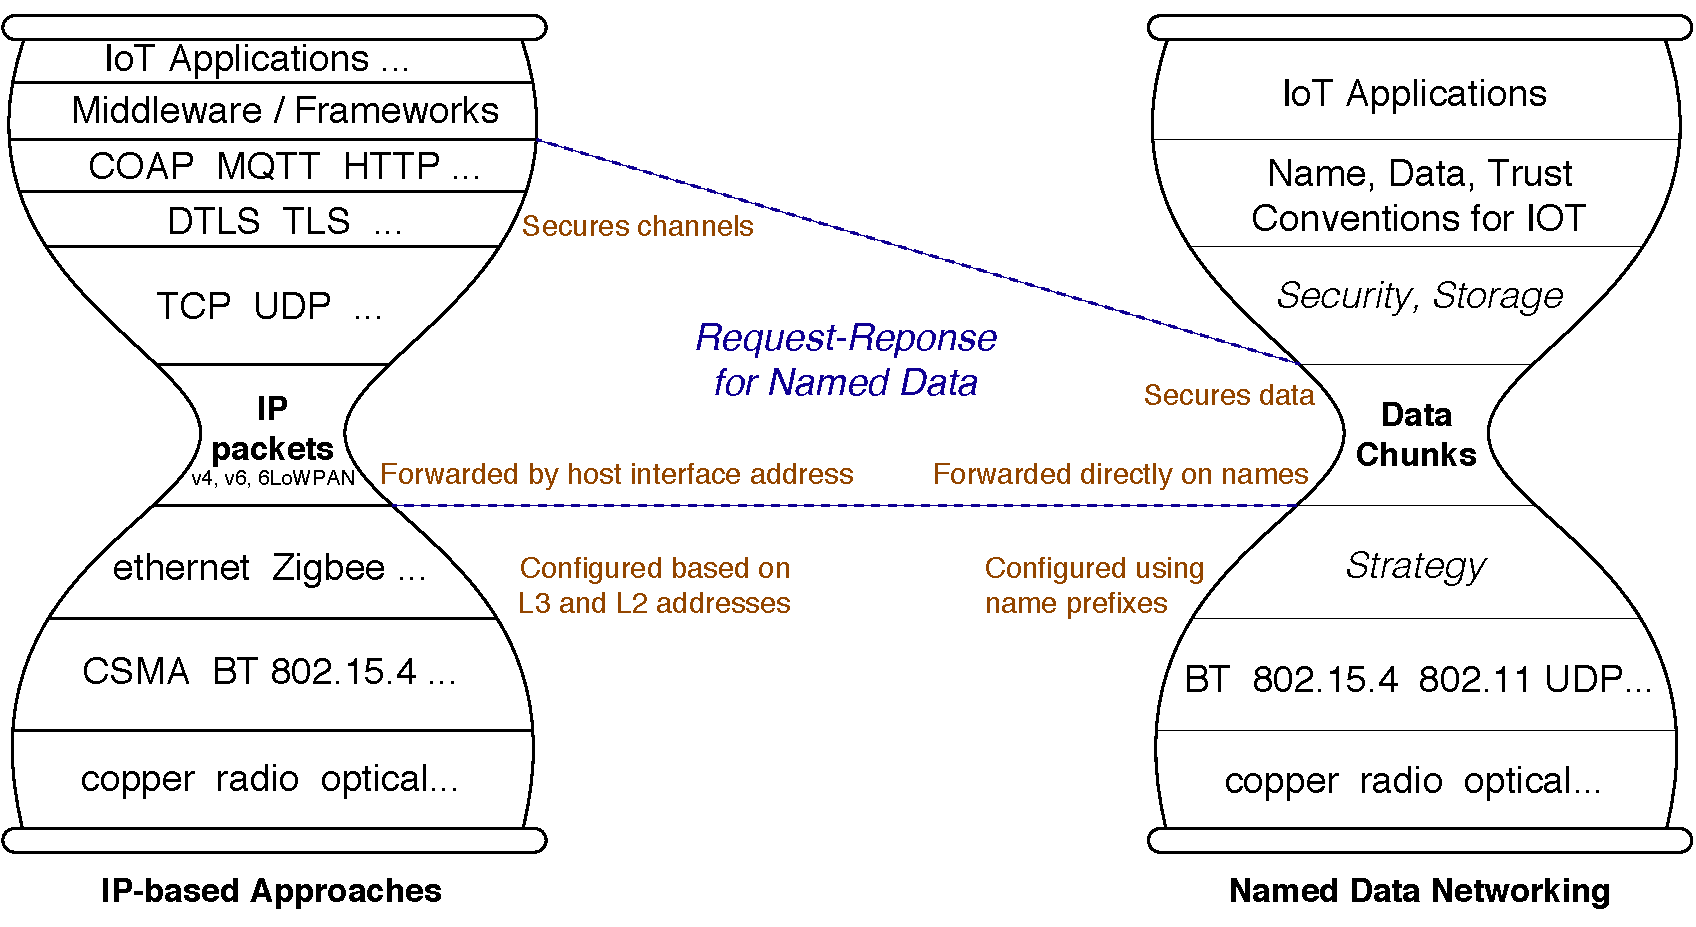
\includegraphics[width=0.9\columnwidth]{ndn-iot-hourglass.pdf}
\caption{Protocol stack comparison of NDN and TCP/IP.}
\label{fig:ndnot-vs-iot}
\end{figure}

The goal of this paper is to demonstrate the design and implementation of a complete IoT system based on NDN, expanding on our previous work.
In particular, we will illustrate how to leverage naming in NDN to achieve trust management and rendezvous in an IoT network, which further enables a variety of IoT applications and services.


% \section{Cloud-independent IoT over NDN}
\label{sec:ndn-iot}

\subsection{IoT and the cloud}
\label{sec:cloud-iot}

IoT applications and services often require a set of common services to be provided by the application-layer frameworks (shown in Fig.~\ref{fig:service-arch}):
\begin{itemize}
\item \emph{Identity management, authentication and authorization}, consisting of trust management for users, devices and services and, in connection-oriented models, access control;
\item \emph{Rendezvous and resource discovery}, enabling applications to find the devices and services they need;
\item \emph{Device management}, to handle onboarding, monitoring, configuration changes, software upgrades, etc. for constituent devices;
\item \emph{Application data messaging}, which supports data exchange through mechanisms including publish-subscribe (pub-sub), streaming, etc.;
\item \emph{Gateways to external network and services}, bridging IoT networks to other services such as data storage and analytics, as well as the public Internet mobile generally.
\end{itemize}

As we discussed in Section~\ref{sec:iot-ecosystems}, most IoT ecosystems today rely on the cloud to implement part or all of those framework services.
For example, in AWS IoT, the Amazon cloud service plays several critical roles that cover all of the above aspects of an IoT platform.
It acts as an identity provider, issuing security credentials for users and devices.  It provides authorization services, whereby device certificate issued by AWS contains the resource access policies prescribed by the user. It handles device management and rendezvous, where all devices in the IoT system register with and report to AWS, which also collects state for all devices and makes it available to applications.  All messages between IoT devices and services are tunneled through the cloud for pub-sub dispatching. AWS can host applications that consume the IoT data and trigger actions when certain events happen. Users can access the IoT network from public Internet, the messages are also tunneled through AWS via the message brokers.  

% The following is an application - 
%AWS IoT can store the device state persistently and analyze the IoT data using a variety of AWS services;

\begin{figure}[!t]
\centering
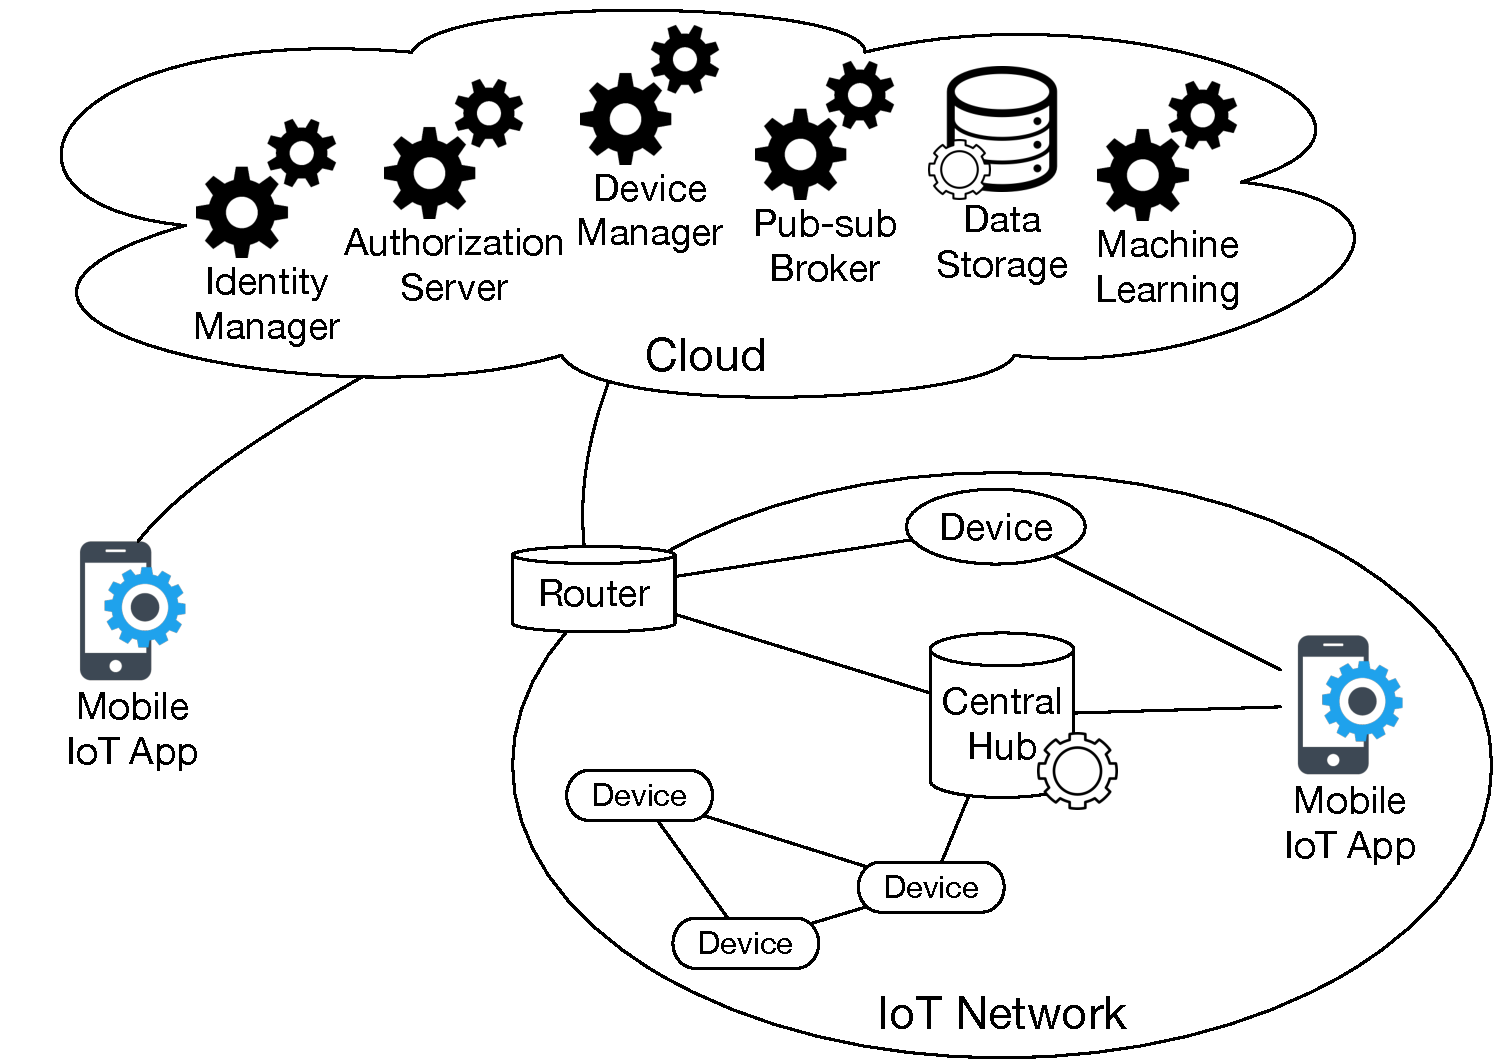
\includegraphics[width=0.9\columnwidth]{cloud-iot.pdf}
\caption{Typical cloud-centric IoT architecture}
\label{fig:cloud-iot}
\end{figure}

A typical cloud-centric IoT architecture is depicted in Fig.~\ref{fig:cloud-iot}.
%The cloud-centric model stems from the technical artifact that TCP/IP networking focuses on connecting different end nodes.
The cloud provides a convenient ``central hub'' for managing and interconnecting a large number of devices. 
While it simplifies the system configuration and management for the users by moving the control into the cloud, a cloud-centric IoT architecture sacrifices the opportunity of exploring proximal communications to achieve better reliability and efficiency.
The connectivity to the remote servers in the cloud becomes a single point of failure that unnecessarily affects the local services in the IoT network, and unnecessarily requires local data traverse the global network.
For example, for home IoT systems, a user cannot install or re-configure devices at home or access home network from public Internet if the connectivity from home to the cloud is down.
In ``human-in-the-loop'' application scenarios, control messages from the user's smartphone are first routed to the cloud for authentication and logging before being forwarded to the IoT device.
This extra latency is damaging for real-time, interactive applications, such as IoT-augmented home entertainment experiences. Further, the exposure of home devices to the global network unnecessarily is a security risk.


% \subsection{Rethinking IoT Service Architecture}

Among the IoT framework services shown in Figure~\ref{fig:service-arch}, two play a more fundamental role:
\begin{enumerate}
\item \emph{Trust management}, which mandates how the IoT system entities (users, devices, and applications) can authenticate each other;
\item \emph{Rendezvous}, which provides a means for different entities to reach each other over the local and global networks.
\end{enumerate}

Independent from the lower layer addressing scheme, trust management and rendezvous at the application layer are built on the concept of \emph{named entities}.
The application-layer names are either specified by the users or auto-generated by the devices and applications.
Those names serve as the \emph{identities} of the entities in an IoT system and allow those entities to refer to each other and interoperate.
To enable authentication, the identity names are usually associated with some form of credentials such as user passwords and public key certificates.
Therefore application-layer trust policies can be composed in terms of names rather than low-level security material.
Named entities also provide the basis for rendezvous: by exchanging names, entities can find out about other entities on the network. 

All other IoT services can be bootstrapped from these two core services.
For example, device management is based on the mutual trust and direct communication (via rendezvous) between devices and managing services;
resource discovery is a natural extension of rendezvous, enhanced by the ability to verify a resource's origin;
pub-sub messaging and external gateways both require the interplay of authentication and rendezvous functions.
Note that those services may also be interdependent on each other; together they form a framework layer on top of which IoT developers can create high-level applications and services.

%Today's cloud-centric IoT ecosystems typically provide most (if not all) of the framework-level and application-level services in Figure~\ref{fig:service-arch}.
A common argument for hosting IoT services and applications in the cloud is that the IoT system would become too complicated for ordinary users if they have to deal with the complexity of registering devices with some local controller, connecting devices with local and remote applications, and managing security credentials.
However, we argue that the usability problem can be addressed fundamentally with a hierarchical and human-friendly naming design because:
(1) human-friendly naming provides intuitive understanding of the trust relationship among devices and applications for non-expert users;
(2) hierarchical naming structure facilitates applications in expressing and exploring the organization of the IoT system, which further enables automated trust management and rendezvous tools.

Unfortunately, in TCP/IP network architecture the first-order names for devices and services are IP addresses,%
\footnote{For example, in cloud computing it is common practice to assign one or more \textit{virtual IPs (VIPs)} to identify cloud services. VIPs are often different from the IP addresses of the physical machines that host the services.}
accompanied by per-device or per-service public keys for (D)TLS authentication.
Human-readable names, such as URLs, are application-layer aliases that have to be resolved when the applications access data or services via the network.
Numeric names are straightforward for machines to operate on, but contain no semantic meaning that can be leveraged to make trust decisions, support rendezvous, or provide intuitive understanding for human users and application developers.
%The numeric names, while easy to handle by the servers in the cloud, are unintuitive for human users and application developers.
The NDN architecture offers an elegant solution to the naming problem at the network layer. It allows the IoT services to be described locally and in a decentralized way without sacrificing security, functionality, flexibility, and usability (described in the next subsection).

\subsection{Achieving Local IoT Functions with NDN}

The NDN architecture bootstraps proximal IoT communication by naming the entities in the context of the local IoT network.
Instead of obtaining their identities from cloud service providers, the entities in the IoT network create local identities associated with asymmetric cryptographic keys that are certified by a local trust anchor.
The identity certificates are all published as Data packets in the local NDN network under the identity namespace.
The trust anchor is typically a root key created by the manager of the IoT system and stored securely on a local authentication server such as a control hub or a TPM-equipped smartphone.
With the support from appropriate tools, the key and certificate management tasks can be made user-friendly enough for non-experts.

Note that the entities may also have other identities for communication outside the IoT network.
For example, the devices may have manufacture-issued identities that are used for signing the device state reports or retrieving software/firmware updates;
the users may also have public identities (e.g., OpenIDs) that can be used for initial authentication when new users are added to the system.
The practice of using different identities for different purposes is aligned with the \emph{principle of least privilege}.

After the local identities are created, the NDN-IoT architecture can leverage two powerful tools to provide the two fundamental services: using \emph{schematized trust}~\cite{trust-schema} for local trust management, and \emph{distributed sync}~\cite{chronosync} for local rendezvous.

\subsubsection{Trust management}
The trust policies for the IoT system can be expressed by the \emph{trust schema}, which specifies the relations between data name and signing key name using a domain-specific language designed for pattern matching on NDN names.
The NDN software platform provides tools that automatically sign and verify the Data packets according to the pre-defined trust schema, which can be integrated into the applications through client libraries.

\subsubsection{Rendezvous}
NDN Sync protocols such as \emph{ChronoSync} allow multiple devices to synchronize the namespace of the shared dataset without relying on central servers.
This mechanism provides a convenient rendezvous solution where the application prefixes and device identities are published under a well-known namespace and synchronized across multiple devices in the IoT network.
For large-scale IoT systems, multiple sync groups can be created under separate namespaces to isolate independent subsystems.

Through support for decentralized trust management and rendezvous, the NDN-IoT architecture enables cloud-independence while providing essential IoT services.
Applications can still benefit from the cloud whenever they need, such as storing large amount of data, performing complex data analysis jobs, or accessing external services like search and voice recognition.
In fact, NDN simplifies the integration with the external networks by using the universal Interest-Data exchange primitive for data communication.
The cloud services become an optional component, rather than the central piece in the architecture.

The automated local trust management and rendezvous also improve user experience because the only manual step of configuration during device setup is to register the device with the local trust anchor and obtain certified local identity for the device.
Once the trust is established, the IoT devices and applications can communicate with each other, exchange useful information, or discover new devices and applications without human intervention.

\section{Flow: a Home Entertainment Experience over NDN}
\label{sec:components}

% Flow: game experience description
In this section, we describe the design of Flow, a home entertainment experience that leverages NDN to realize a cloud-independent, IoT-supported application. We conclude by summarizing the components of a generalized NDN-IoT framework developed based on this design.
Flow is a prototype of a multi-user ``exploration game'', in which participants navigate and interact with a virtual world rendered in a game engine using a combination of inputs: 
\begin{enumerate}
\item \textit{Indoor positioning}: participants' positions in physical space, detected by indoor positioning (person tracking), modify the virtual landscape;
\item \textit{Wearable sensing}: participants directly control orientation of the environment's virtual camera using gyroscopes connected to  microcontrollers, which can be worn or carried; 
\item \textit{Mobile phone interface}: participants interact with the virtual environment through controls on their smartphone, for example to share social media images in the virtual environment.
\end{enumerate}
In addition to various types of IoT devices and the game engine, the system on which Flow is built also includes an \textit{authentication server} (AS) that performs local trust management.
The AS can be implemented as an app on the owner's smartphone, or a service daemon on a dedicated control hub (e.g., the home router).

\begin{figure}[!t]
\centering
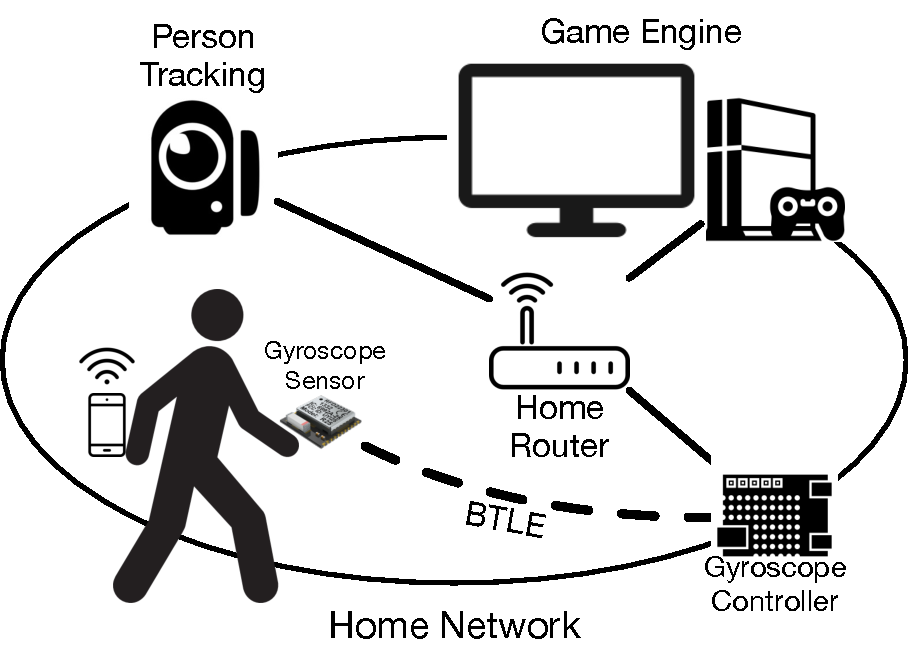
\includegraphics[width=0.9\columnwidth]{flow-home-deployment.pdf}
\caption{Typical deployment of the Flow home entertainment experience.}
\label{fig:flow-deployment}
\end{figure}

% Flow features: cloudless, security, an integrated solution with different types of devices and sensing
%Flow adopts a cloudless architecture, and uses the NDN protocol stack to connect hardware with varying capabilities, as well as secure a diverse range of sensing data. The rest of this section introduces how this is achieved from the perspectives of namespace, bootstrap and trust relationship, and device discovery using synchronization.

Figure~\ref{fig:flow-deployment} shows a typical deployment scenario of Flow in a home network.  NDN interconnectivity between different components is supported over Ethernet and Wi-Fi, through the home Wi-Fi router in a hub-and-spoke topology. 

Sensor devices with limited networking capability (e.g., the gyroscope in Fig.~\ref{fig:flow-deployment}) may be bridged via a helper device.
We assume all devices can reach each other over NDN, which is trivial in a hub-and-spoke topology.\footnote{A routing protocol may be required if a sensor mesh topology is deployed inside the home network.}

\subsection{Naming and Identity}
\label{sec:naming}

% Design: namespace
In Flow, data from the IoT \textit{things} used by the application are named using three namespaces:
\begin{itemize}
\item \emph{Application namespace}: a local namespace for publishing and accessing application data, e.g., gyroscope readings needed to control the environment; 
\item \emph{Device namespace:} a local namespace for publishing device identity certificates and metadata;\footnote{Device metadata could include information about devices and their capabilities as well as bindings to application names.}
\item \emph{Manufacturer namespace}: a global namespace created by the IoT device vendors and for trust bootstrapping.
\end{itemize}


Fig.~\ref{fig:flow-namespace} shows an example of the Flow namespace.  In addition to these three namespaces which names devices, things and their data, note the \textit{discovery} branch under the local root prefix, which is used for device rendezvous and for application prefix discovery. Details of its functionality are described later.


\begin{figure*}[!t]
\centering
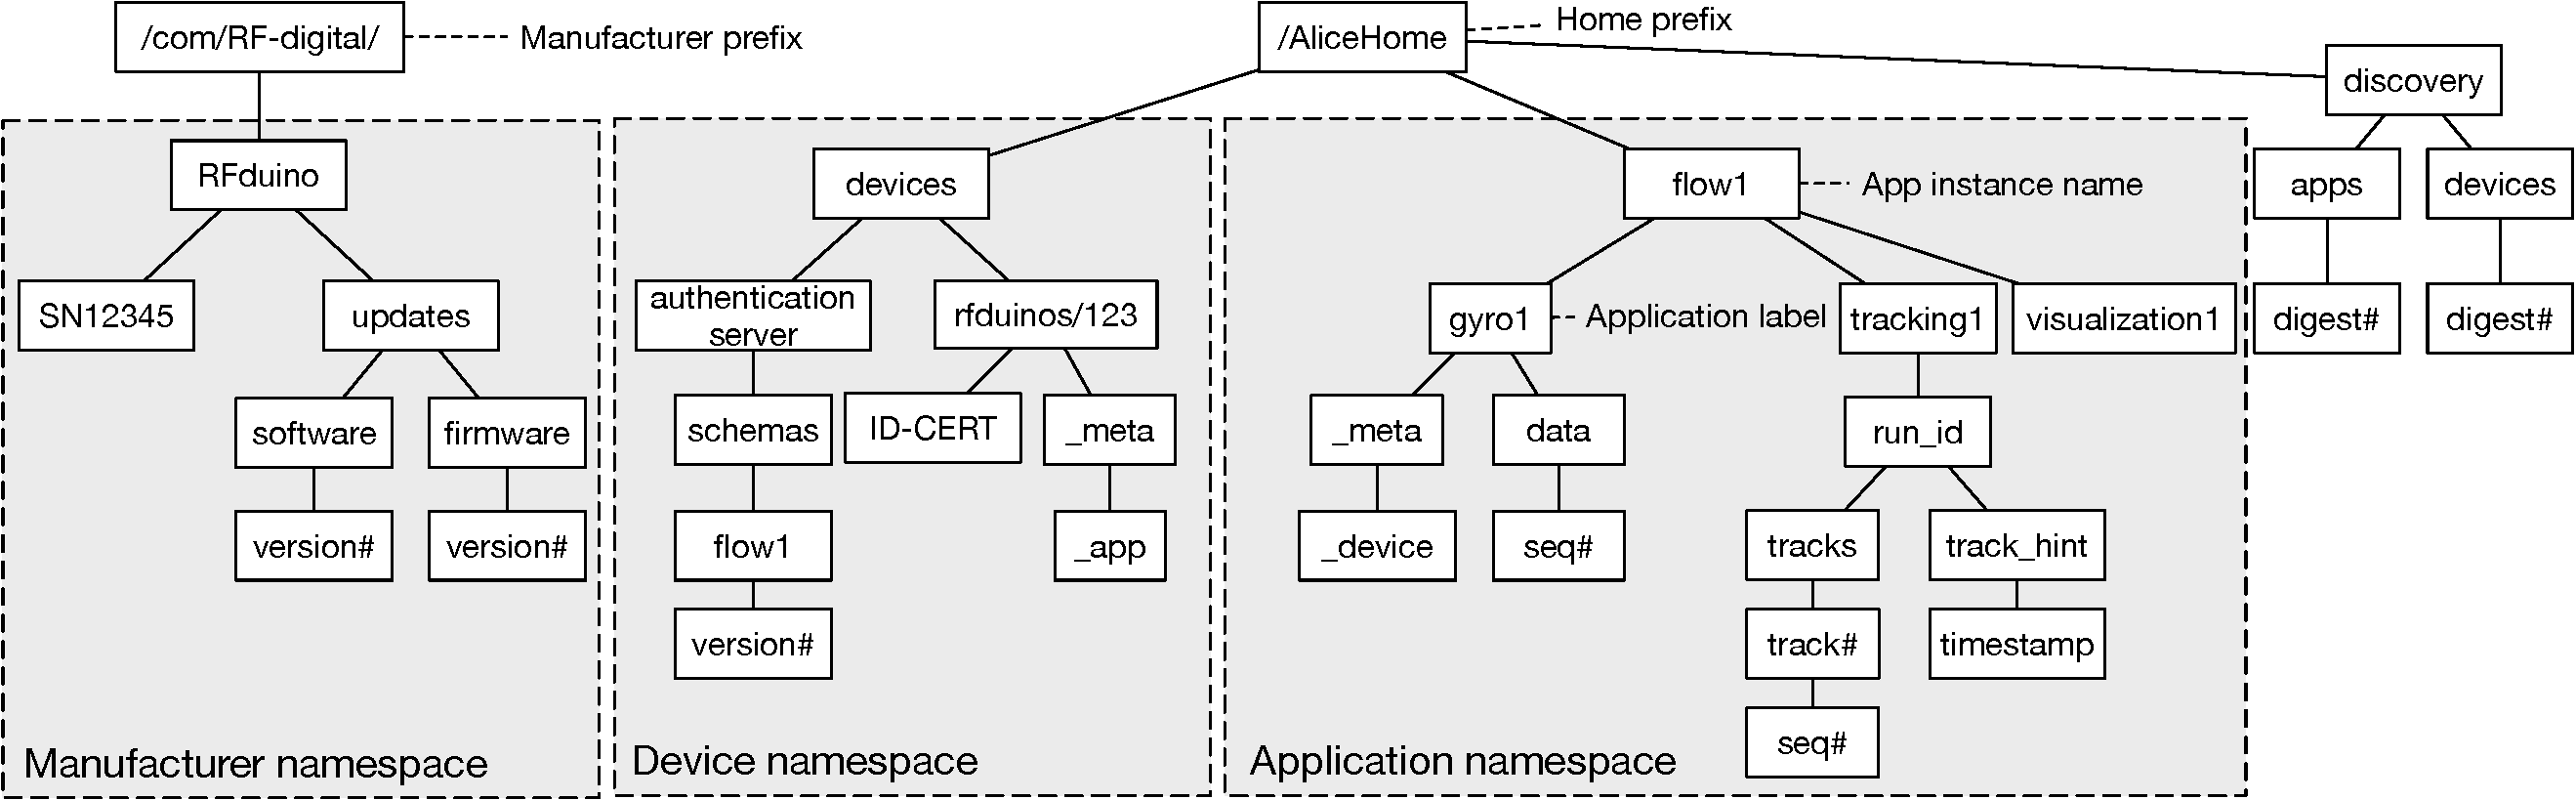
\includegraphics[width=0.95\textwidth]{flow-namespace.pdf}
\caption{Example namespace within the home environment where Flow is deployed.}
\label{fig:flow-namespace}
\end{figure*}

The device and application namespaces both have as their root a home prefix that is either context-dependent (e.g., \ndnName{/AliceHome} as in Fig.~\ref{fig:flow-namespace}) or globally reachable (e.g., \ndnName{/att/ucla/dorm1/301}).

The application namespace starts with a unique instance name (e.g., \ndnName{/AliceHome/flow1}) created by the application at installation. 
Data produced by each component is named under an application label configured by the developer (e.g. \ndnName{/AliceHome/flow1/tracking1}). The application label also contains a metadata subtree containing the device name that serves this data (e.g. \ndnName{/AliceHome/flow1/tracking1/_meta/_device}).

Devices publish their local identity certificates under the device namespace (e.g., \ndnName{/AliceHome/devices}).
They also publish metadata (profile) information in the \ndnName{_meta/_app} branch under the device identity prefix to list the application data prefixes they are publishing under. 
The device namespace of an AS also contains the trust schema of currently active applications. 
Schema and trust relationship details are described later in this section.
%JB: Should reference anything in 2016 paper? 

The manufacturer namespace falls under vendor-specific prefixes that are independent from the home network's local prefix.  We envision that manufacturers will have globally unique names for their products used during  bootstrapping, over-the-air updates, and similar processes. 
Manufacturers publish their own certificates under this globally unique prefix so that the devices can authenticate the data coming from the vendors such as software/firmware updates and service notifications.\footnote{Reachability of data in this prefix is not addressed here but can be accomplished through encapsulation supported by the home router, for example.}
In the research example of Flow, all devices are configured with vendor-provided identity names and profiles in their initial provisioning, before being connected to the home network. These are used for device onboarding.

\subsection{Trust Management}
\label{sec:trust-management}

Flow demonstrates a multi-step process for trusting new devices in a home IoT network and enabling their data to be used in an application.  First, a device is assigned a device-level name and added to the trust hierarchy for things in the home. Then, it is configured with one or more application-level names for its data, and these names are added to application trust hierarchies. Finally, the device is configured to respond to requests in application namespaces. 

%The first step of introducing a new device or user to the Flow system is to establish the trust relationship between the device/user and the existing entities in the system.
The authentication server acts as the trust anchor. It can be coordinated with but does not depend on a remote cloud services.
While the devices and users may have public identities outside the home environment, they all need to obtain local identities that are certified by the AS before they can start interacting with other local entities.\footnote{The public identities may be used to assist the onboarding process, but will not be required for local communication once the initial configuration has finished.
For example, a new user can authenticate with the AS using her public identity (e.g., OpenID or Google/Facebook account) before creating her local identity that is used solely by the home environment.}

The process of establishing a trust relationship between a new device and the home through the AS is similar to the Bluetooth pairing process.
To bootstrap a new device, the user---or a configuration application on his/her behalf---provides a shared secret and a local device name.  The shared secret may be a device barcode, identity communicated by NFC, or simply a PIN number. 
The AS sends a command Interest to the device, signed using a key derived from the shared secret, to ask that it generate a public/private key pair associated with the device's new name on the local network.  The device replies with a Data packet containing an identity certificate request, also signed by the shared secret.
The AS generates the identity certificate based on this request.  The device, now part of the trust hierarchy, can advertise its services or participate in an application over the local network.
This process is illustrated in Fig.~\ref{fig:flow-bootstrap}.
If the device has been issued a public identity certificate by its vendor, the AS may optionally authenticate its public identity, e.g., by asking the device to sign an AS-generated challenge.


\begin{figure}[!t]
\centering
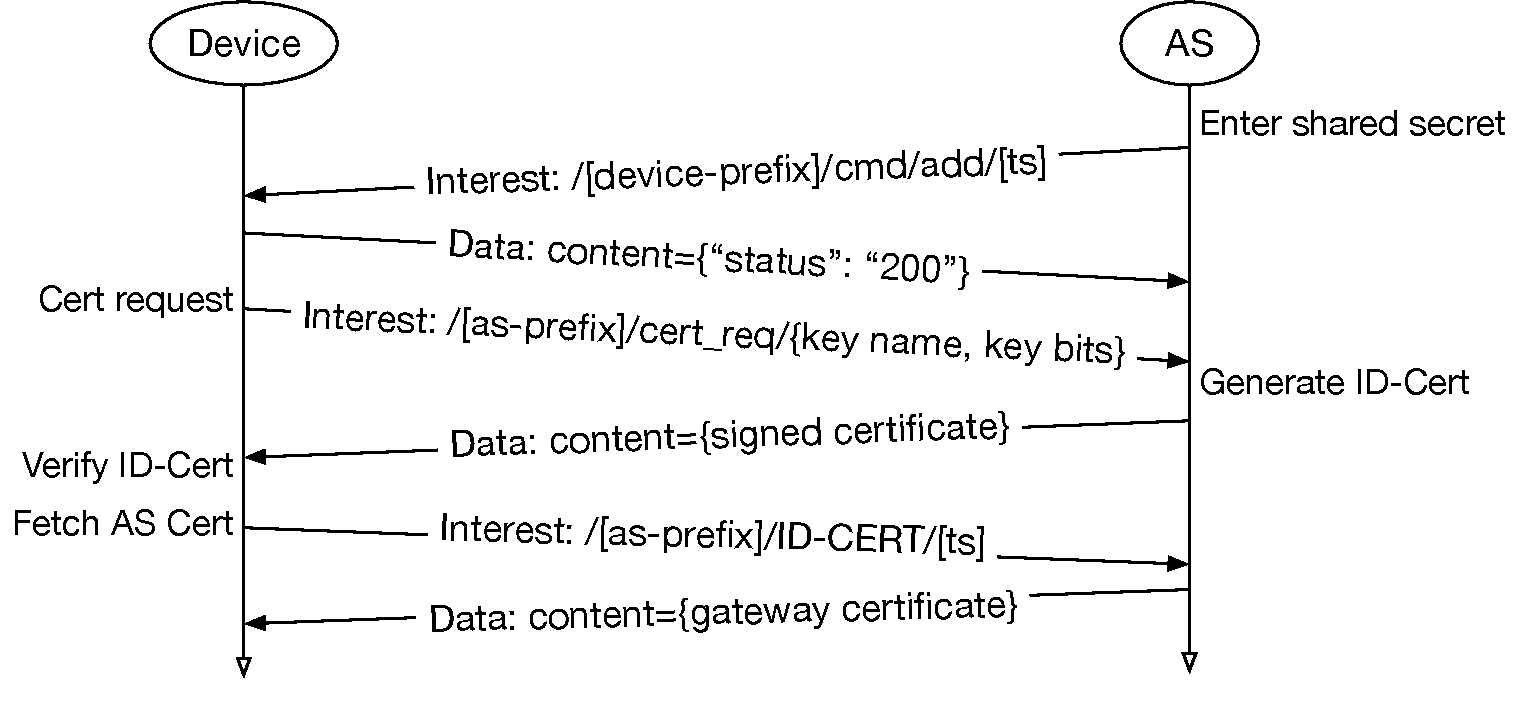
\includegraphics[width=0.95\columnwidth]{add-device-sequence.pdf}
\caption{Bootstrap trust relationship for new device.}
\label{fig:flow-bootstrap}
\end{figure}

Applications like Flow are ``installed'' in a similar way to devices, with the AS signing both identity certificates and trust schema for the application.  The application's trust schema  expresses \textit{what devices identities are authorized to publish under what application prefixes} and is published as a normal Data object on the local NDN network.  For example, in Fig.~\ref{fig:flow-namespace} \ndnName{flow1} is a specific Flow instance and \ndnName{schema} branch contains the trust schema of this instance.
The schema name includes a monotonic version number at the end, so when there is a change in the schema a newer version is published.
The technical details of how to specify a trust schema are described in~\cite{trust-schema}.
% Other device names in the example include an ``RFduino'' device, which in ``flow1''publishes for the gyroscope ``gyro1'' that it's physically connected to. Under a device name a ``\_meta'' branch is introduced, in which the device can list under what application prefixes it's publishing. Two other subsystems of the game, person tracking (``opt1'' branch) and visualization (``unity'' branch) are featured in the example namespace.

%Applications like Flow can request that devices publish data under application-level namespaces by issuing command Interests to them.   The device evaluates the request according to the available trust schema. 

% Design: trust - application producer authorization
When a device that produces data is installed, it sends a command Interest to the AS that includes the application prefix it intends to publish under and its own local identity.
If the request to publish data in the home network is granted, the AS will update the trust schema with the authentication rules for data published by this device. The rule binds a device identity with the application prefixes it's authorized to publish under.\footnote{This binding addresses potential collision in application labels--for example, by default the AS does not authorize a second device to publish under an application namespace claimed by another.}
Schematized trust enables fine-grained control over what devices can publish what data for which application instances. Consumer devices fetch the latest trust schema over the network via NDN and follow the rules to authenticate the data packets published in the network.
The producer authorization process, as well as an example of the resulting trust relationship, is shown in Fig.~\ref{fig:flow-app-authorization-trust-relationship}, in which the AS signs a device identity, and the device signs a piece of application data it publishes.

\begin{figure}[!t]
\centering
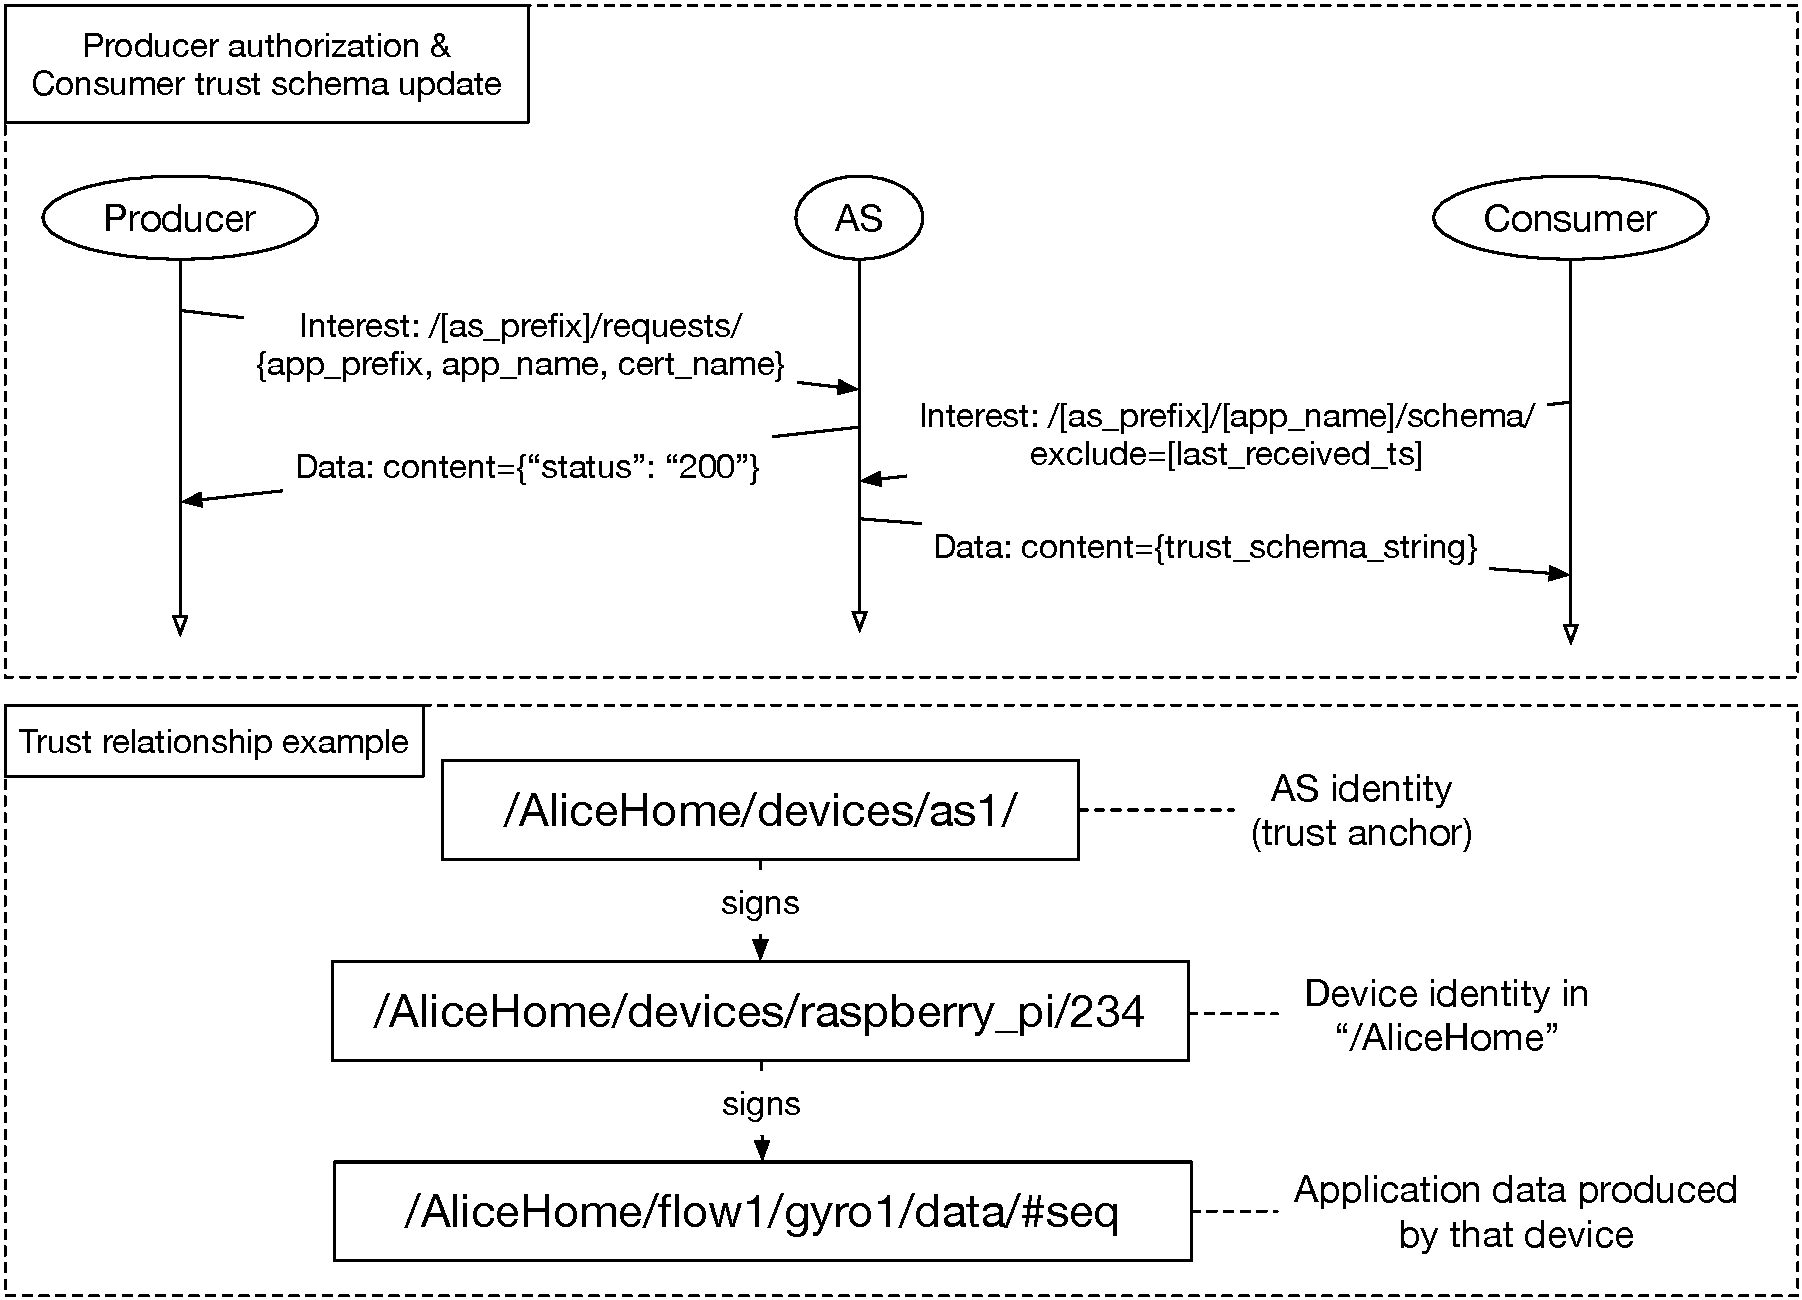
\includegraphics[width=0.95\columnwidth]{authorize-producer-consumer.pdf}
\caption{Schematized trust between producers and consumers.}
\label{fig:flow-app-authorization-trust-relationship}
\end{figure}


\subsection{Rendezvous}
\label{sec:rendezvous}

% Design: discovery (chronosync recovery)
%Each subsystem in Flow needs to learn the application names of other subsystems in order to communicate with them. For this purpose device discovery is introduced. Discovery exchanges messages in ``/home/devices/discovery'' namespace as shown in Fig.~\ref{fig:flow-namespace}, similar to ChronoSync's \cite{chronosync}, a digest of this device's currently known names is attached to the interest name. Receivers of this interest, upon seeing a different digest, will reply with its own set of names. Differing from the suggestion in \cite{ndn-iot}, This synchronization-based discovery is introduced so that any device in the home can help answering a discovery interest, and the controller, after registering the devices and serving required certificates, can stay offline.

Flow also demonstrates a name-based, distributed rendezvous mechanism for devices and applications to discover each other over NDN.
As described in the previous section, The key idea is to synchronize the set of device and application names (called the \textit{rendezvous dataset}) across nodes in the network that are interested in learning about them.
The synchronization process utilizes the decentralized and serverless ChronoSync~\cite{chronosync} protocol to effectively synchronize prefixes of active devices under the home entertainment \ndnName{/AliceHome/discovery/devices} namespace.
% When a device receives a digest different from its own, it replies with a Data packet containing its own set of names.
% Recipients of these replies merge the received dataset with their own local ones.
% Eventually all participating devices will reach agreement about the rendezvous dataset, provided that the configuration changes more slowly than the necessary messages can be exchanged. %system is able to stay in a stable state with no frequent configuration changes.
% This protocol does not require assistance from a central server either locally or remotely.

Name discovery is performed independently on each device by lookups in the local copy of the rendezvous dataset.
% JB: How? Is this an API call? 
Once an application obtains the name prefix of the target device or application, the devices can follow the namespace structure described in~\ref{sec:naming} to construct Interests for fetching the certificates and metadata, which will bootstrap high-level service communication.

%%  JB:  I don't understand this section - seems like it should be rewritten in the context of the IOTDI paper? 

\subsection{Generalizing IoT functionality in NDN}

Through the design of Flow, we explored how to use NDN to provide the functionality discussed in section~\ref{sec:cloud-iot} without reliance on any cloud services, and generalized it in a framework called \textit{NDN-IoT}, which provides the following features: 

\begin{itemize}

\item \textit{Identity, authentication and authorization}: each device in NDN-IoT possesses two identities: a manufacturer-given name used before and during device onboarding, and a local device name used afterwards. NDN-IoT implements mechanisms described in sections~\ref{sec:naming} and ~\ref{sec:trust-management} for naming, data authentication and device authorization. 
% Repetition and no close connection...

\item \textit{Rendezvous and resource discovery}: nodes in NDN-IoT find the name prefixes of other devices, applications and services in \textit{discovery} namespace via distributed dataset synchronization, and then uses discovered names to fetch devices and applications data, or invoke services in the local system. 
% Repetition of the same thing in the last paragraph of Rendezvous

\item \textit{Device management}: NDN-IoT performs device onboarding and software updates in manufacturer namespace, and device monitoring in device namespace. 
% More non-trivial things to say about this?

\item \textit{Application data messaging}: NDN-IoT provides application-level pub-sub under two types of namespace abstractions. The framework pipelines interest for data named in a \textit{sequence number namespace} (e.g. \ndnName{/AliceHome/flow1/gyro1/data/[sequence_number]}), or keeps outstanding interest for data named in a \textit{timestamp namespace} (e.g. \ndnName{/AliceHome/devices/pc1/_status/[timestamp]}).

\item \textit{Gateways to external network and services}: the local IoT system can request data from the global Internet using their public names, meanwhile its local data can be made available to the public Internet by using a globally reachable name prefix, or having a gateway device that uses data named under a globally reachable prefix to encapsulate data from the local system (e.g. \ndnName{/att/ucla/dorm1/301/flow1/gyro1/data/1} $\rightarrow$ \ndnName{/AliceHome/flow1/gyro1/data/1}).

\end{itemize}



\section{Implementation}
\label{sec:implementation}

We implemented the NDN-IoT framework and a prototype of Flow application separately.
This section describes details in both the framework and application components.

\subsection{NDN-IoT framework}

The NDN-IoT framework is a set of libraries in Python, C++, JS and C\# built on top of the NDN Common Client Libraries.
Each library in the framework implements the naming, trust management and rendezvous in Section~\ref{sec:components} from three functional blocks: bootstrap, discovery and application-level pub/sub.
The overall structure of the framework is shown in Figure~\ref{fig:ndn-iot-framework-structure}.

\begin{figure}[!t]
\centering
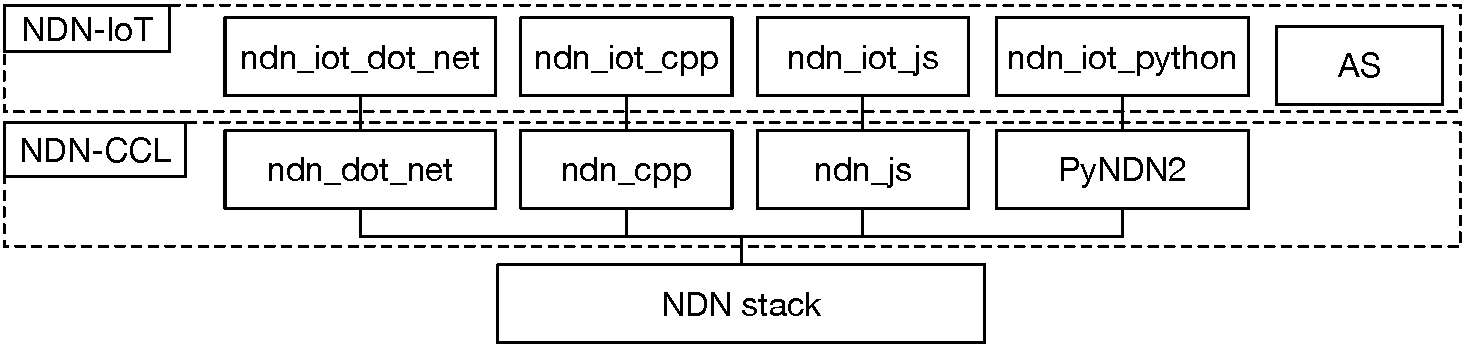
\includegraphics[width=0.95\columnwidth]{ndn-iot-structure.pdf}
\caption{The structure of NDN-IoT framework.}
\label{fig:ndn-iot-framework-structure}
\end{figure}

The rest of this subsection covers each functional block, and a description of the AS implementation available in Python and JavaScript.

% AS
The AS functionality is implemented based on the team's previous work on NDN-pi (citation: ndn-pi TR).
The framework provides a server implementation in Python, which we run on Raspbian platform in Flow application.
The server implementation also updates the codebase to work with PyNDN2 2.0b4, with major updates to security module interface, including using CCL library's built-in public/private key storages. \footnote{We now use BasicIdentityStorage and FilePrivateKeyStorage for key storage, and ConfigPolicyManager for data verification, whereas the old implementation, developed at a time when PyNDN security library module was evolving, used custom derived classes (for example, IotPrivateKeyStorage).}
Authentication clients are available in both Python and JavaScript in order to support application components running on Ubuntu, OSX, Raspbian, and browser (Chrome and Firefox) platforms.
Compared with the earlier work in NDN-pi, this implementation added a port in JavaScript to support browser applications. 
The JavaScript port uses the library's IndexedDbIdentityStorage and IndexedDbPrivateKeyStorage for key storage (this means the key storage in browser is origin-based, thus in our installation the webpage that adds this ``device'' and the webpage that publishes application content should be hosted under the same origin). 
Recall that in NDN-pi the client device generates a device ID\footnote{The server uses this ID to construct the initial ``add device'' interest name. This ID was implemented as the CPU serial of a Raspberry Pi.}. 
In browser application's case we generate a random string in IndexedDB if one doesn't already exist, to use as the device identification of the device that currently runs the browser.

% NDN-IoT client libraries

\textbf{Bootstrap} follows the suggestion in section VI.B and VI.C of the IoTDI '16 paper, and helps with device and application identity setup. Its abstractions include: 
\begin{enumerate}
\item KeyChain setup: given a device identity (and optionally an AS name), construct a KeyChain and set up the default device certificate name for this application instance. This KeyChain is later used for signing and verification of all application data.
\item Consumer setup: given an application prefix, the Bootstrap module keeps outstanding interest for the application's trust schema (add example), and updates the local copy whenever a later version is received and verified.\footnote{The application trust schema may evolve over time, when new device names are added and authorized to publish under certain application prefixes}
\item Producer setup: given an application prefix, the Bootstrap module requests authorization from the AS to publish under that prefix by sending a command interest including this device's identity and the prefix it wants to publish for (add example). If the AS authorizes the request, it adds an entry stating to the application trust schema to reflect the updated trust relationship, and publishes a new version for all consumers to fetch.
\end{enumerate}

In practice, the application code to set up a gyroscope data producer on a Raspberry Pi may look like the following.
\begin{minted}
[frame=lines,
framesep=2mm,
baselinestretch=1,
fontsize=\footnotesize,
breaklines
]{python}
from ndn_iot_python import Bootstrap
deviceName = Name("/AliceHome/devices/rpi2")
dataPrefix = Name("/AliceHome/flow1/gyros")
appName = "flow1"
face = Face()
bootstrap = Bootstrap(face)
bootstrap.setupDefaultIdentityAndRoot(deviceName, onSetupComplete, onSetupFailed)

def onSetupComplete(certificateName, keyChain)
  bootstrap.requestProducerAuthorization(dataPrefix, appName, onRequestSuccess, onRequestFailed)

def onSetupFailed(message)
  print(message)
\end{minted}

And in a Flow application instance ``flow1'', a trust schema built by the AS may contain the following sections.
\begin{minted}[frame=lines,
framesep=2mm,
baselinestretch=1,
fontsize=\footnotesize,
breaklines
]{text}
trust-anchor 
{
  type "base64"
  base64-string "Bv0DD..."
}
\end{minted}
Trust anchor certificate is installed during the bootstrap process.
This rule is automatically populated by the AS.

\begin{minted}[frame=lines,
framesep=2mm,
baselinestretch=1,
fontsize=\footnotesize,
breaklines
]{text}
rule 
{
  id "Certs"
  for "data"
  filter 
  {
    type "regex"
    regex "^[^<KEY>]*<KEY><>*<ID-CERT>"
  }
  checker 
  {
    type "customized"
    sig-type "rsa-sha256"
    key-locator 
    {
      type "name"
      name "/AliceHome/devices/gateway/KEY/ksk
-1485314801/ID-CERT"
      relation "equal"
    }
  }
}
\end{minted}
This rule mandates that all certificates should be signed by the gateway.\footnote{In this iteration of Flow, device certicates are the only type of certificate involved in the trust relationship in Section~\ref{sec:trust-management}.}
This rule is automatically populated by the AS.

\begin{minted}[frame=lines,
framesep=2mm,
baselinestretch=1,
fontsize=\footnotesize,
breaklines
]{text}
rule 
{
  id "discovery-data"
  for "data"
  filter 
  {
    type "regex"
    regex "^[^<discovery>]*<discovery><>*"
  }
  checker 
  {
    type "customized"
    sig-type "rsa-sha256"
    key-locator 
    {
      type "name"
      regex "^[^<KEY>]*<KEY><>*<ID-CERT>"
    }
  }
}
\end{minted}
This rule mandates that all discovery data should be signed. 
This rule is automatically populated by the AS.

\begin{minted}[frame=lines,
framesep=2mm,
baselinestretch=1,
fontsize=\footnotesize,
breaklines
]{text}
rule 
{
  id "/AliceHome/flow1/gyros"
  for "data"
  filter 
  {
    type "name"
    name "/AliceHome/flow1/gyros"
    relation "is-prefix-of"
  }
  checker 
  {
    type "customized"
    sig-type "rsa-sha256"
    key-locator 
    {
      type "name"
      name "/AliceHome/devices/rpi2/KEY/dsk-
1485374576/ID-CERT"
      relation "equal"
    }
  }
}
\end{minted}
This rule mandates that data under application prefix \ndnName{/AliceHome/flow1/gyros} should be signed by device \ndnName{/AliceHome/devices/rpi2}.
This rule is added to the trust schema after the AS approves the request from \ndnName{/AliceHome/devices/rpi2}.

\textbf{Discovery} uses a simple sync-based discovery similar to ChronoSync recovery mechanism.

In practice, after setting up the Bootstrap object, the application may use the following code to include a discovery module.
\begin{minted}[frame=lines,
framesep=2mm,
baselinestretch=1,
fontsize=\footnotesize,
breaklines
]{python}
from ndn_iot_python import Discovery, Observer

class MyObserver(Observer):
  def onDiscovered(name, description):
    print(name.toUri() + description)

keyChain = bootstrap.getKeyChain()
certName = bootstrap.getDefaultCertificateName()
syncPrefix = Name("/AliceHome/discovery/devices")
discovery = Discovery(face, keyChain, certName, syncPrefix, MyObserver())

description = "My Raspberry Pi device"
deviceName = Name("/home/devices/rpi2")
discovery.publishObject(deviceName, description)
\end{minted}

\textbf{Application-level pub/sub} follows the suggestion in section VI.F of the IoTDI '16 paper, and provides the following abstractions:
\begin{enumerate}
\item Consumer for timestamp namespace (/prefix/[timestamp]): this consumer uses oustanding interest with range exclusion to ask for latest piece of data, and upon data retrieval and successful verification, updates the range exclusion with the received timestamp.
\item Consumer for sequence-number namespace (/prefix/[sequence-number]): this consumer pipelines interest for the next few sequence numbers, and upon data retrieval and successful verification, issues an interest for the sequence number after the last one in the pipeline.
\end{enumerate}

In practice, after setting up the Bootstrap object, the application may use the following code to include a sequence number consumer module.

\begin{minted}[frame=lines,
framesep=2mm,
baselinestretch=1,
fontsize=\footnotesize,
breaklines
]{python}
from ndn_iot_python import AppConsumerSequenceNumber
keyChain = bootstrap.getKeyChain()
pipelineSize = 5
consumer = AppConsumerSequenceNumber(face, keyChain, pipelineSize)
prefix = Name("/home/flow1/gyros")
consumer.consume(prefix, onData, onTimeout, onVerifyFailed)
\end{minted}

\subsection{Flow application components}

% Subsystems
In our application prototype, each of the components is implemented as the following:
\begin{enumerate}
\item \textit{Indoor positioning}: We use OpenPTrack,\footnote{\url{http://openptrack.org/about/}} a multi-camera person tracking system.
The NDN producer for OpenPTrack\footnote{\url{https://github.com/OpenPTrack/ndn-opt/}} (written in C++)  publishes the position of each person at a 30Hz rate, along with lower rate metadata about active tracks. 
% Interest pipelining and an application-level Pending Interest Table are used for real-time delivery of position data.
% Dealing with constrained devices: better in design or implementation? deserve its own paragraph and figure?
\item \textit{Wearable sensing}: We use an RFduino 22301 with gyroscope MPU6050 attached to provide virtual camera control. 
The RFduino cannot perform asynchronous signing operations quickly enough, so we introduced a Raspberry Pi controller as a gateway for bridging RFduino to the NDN home network.
The data exchanged between RFduino and Raspberry Pi is signed with a shared secret key negotiated after Bluetooth pairing.
The Raspberry Pi generates a public/private key pair on behalf of the RFduino to be associated with the RFduino's device identity.
The RFduino runs a minimum NDN producer, implemented with the ndn-cpp-lite library\footnote{\url{https://github.com/named-data/ndn-cpp/}}, which generates data at roughly 2Hz rate.
When new data is generated, the RFduino pushes the data (signed by the pre-negotiated shared secret) to the Raspberry Pi controller over the Bluetooth LE channel.
The controller receives the data, repackages the data and signs the data using RFduino's private key, and then publishes the data on the home network.
The RFduino data publishing process is shown in Fig.~\ref{fig:contrained-devices-bootstrap}.
% More reasons needed for matching between IDs?
\item \textit{Mobile phone interface}: We employ an Android phone that loads a control webpage (written in JavaScript) in a mobile browser to interact with the virtual environment. 
The phone sends out two types of command Interests: the first one matches an OpenPTrack track ID with that of the mobile, and the second one drops an image onto the virtual environment where the user's avatar is standing. ID matching is introduced so that the visualization knows the location of the user's avatar (identified by a track ID) when an image drop command Interest is issued by the same user (identified by the mobile's ID).
\item \textit{Visualization}: We use the Unity3D\footnote{\url{https://unity3d.com}} game engine for visualization.
The game engine runs C\# NDN data consumers that receive person tracking and virtual camera control data, and a producer that receives image dropping command Interests from the mobile web interface.
\end{enumerate}

\begin{figure}[!t]
\centering
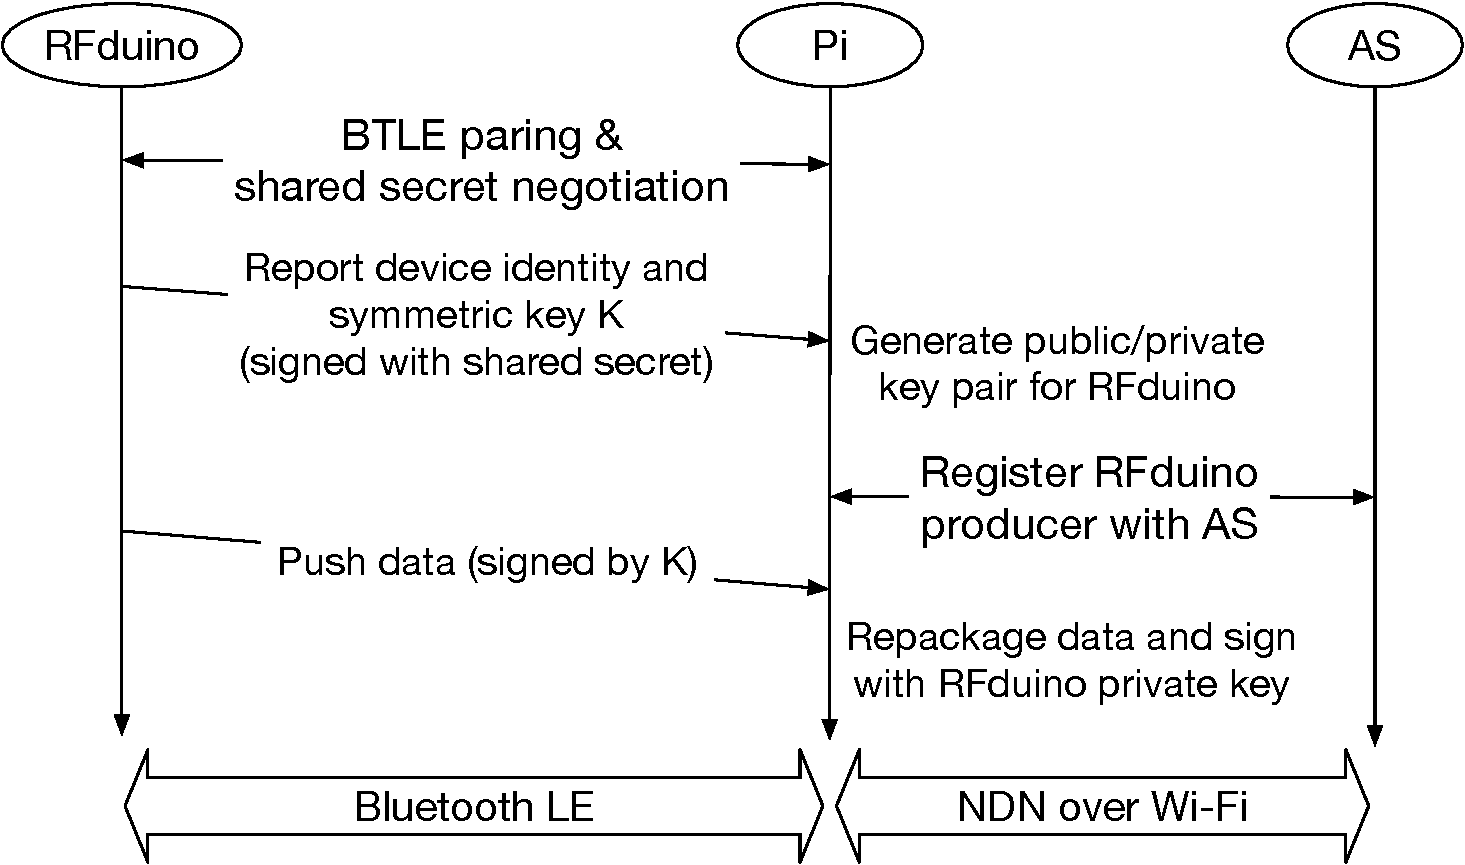
\includegraphics[width=0.95\columnwidth]{constrained-device-authorization.pdf}
\caption{RFduino data publishing with assistance of Raspberry Pi controller}
\label{fig:contrained-devices-bootstrap}
\end{figure}

The implementation for both NDN-IoT framework and Flow application are available online.\footnote{\url{https://github.com/remap/ndn-flow}} We installed two instances of the Flow application testbed at UCLA and Huawei. Fig.~\ref{fig:message-flow-in-flow-installation} shows a diagram of the system and its message flows after all devices are bootstrapped with an AS, which in our installation is another Raspberry Pi.

\begin{figure*}[!t]
\centering
\includegraphics[width=0.95\textwidth]{flow-components-ndn-names-diagram-zs.pdf}
\caption{Application components and message flows in Flow}
\label{fig:message-flow-in-flow-installation}
\end{figure*}




% \section{Evaluation}
\label{sec:eval}

In this section we present a qualitative evaluation that compares Flow and the NDN-IoT framework with the conceptual implementations of a similar gaming system over AWS IoT and Apple HomeKit (using TCP/IP architecture).
The goal of this side-by-side comparison is to highlight the differences between the proposed architecture and the current practice in the industry, and point out how the NDN architecture simplifies the design and implementation of a cloud-independent IoT system.
Fig.~\ref{fig:compare-ecosystems} shows three different designs of home entertainment system over AWS IoT, Apple HomeKit, and NDN-IoT, respectively.

\begin{figure*}[!t]
\centering
\subfloat[Conceptual system over AWS IoT]{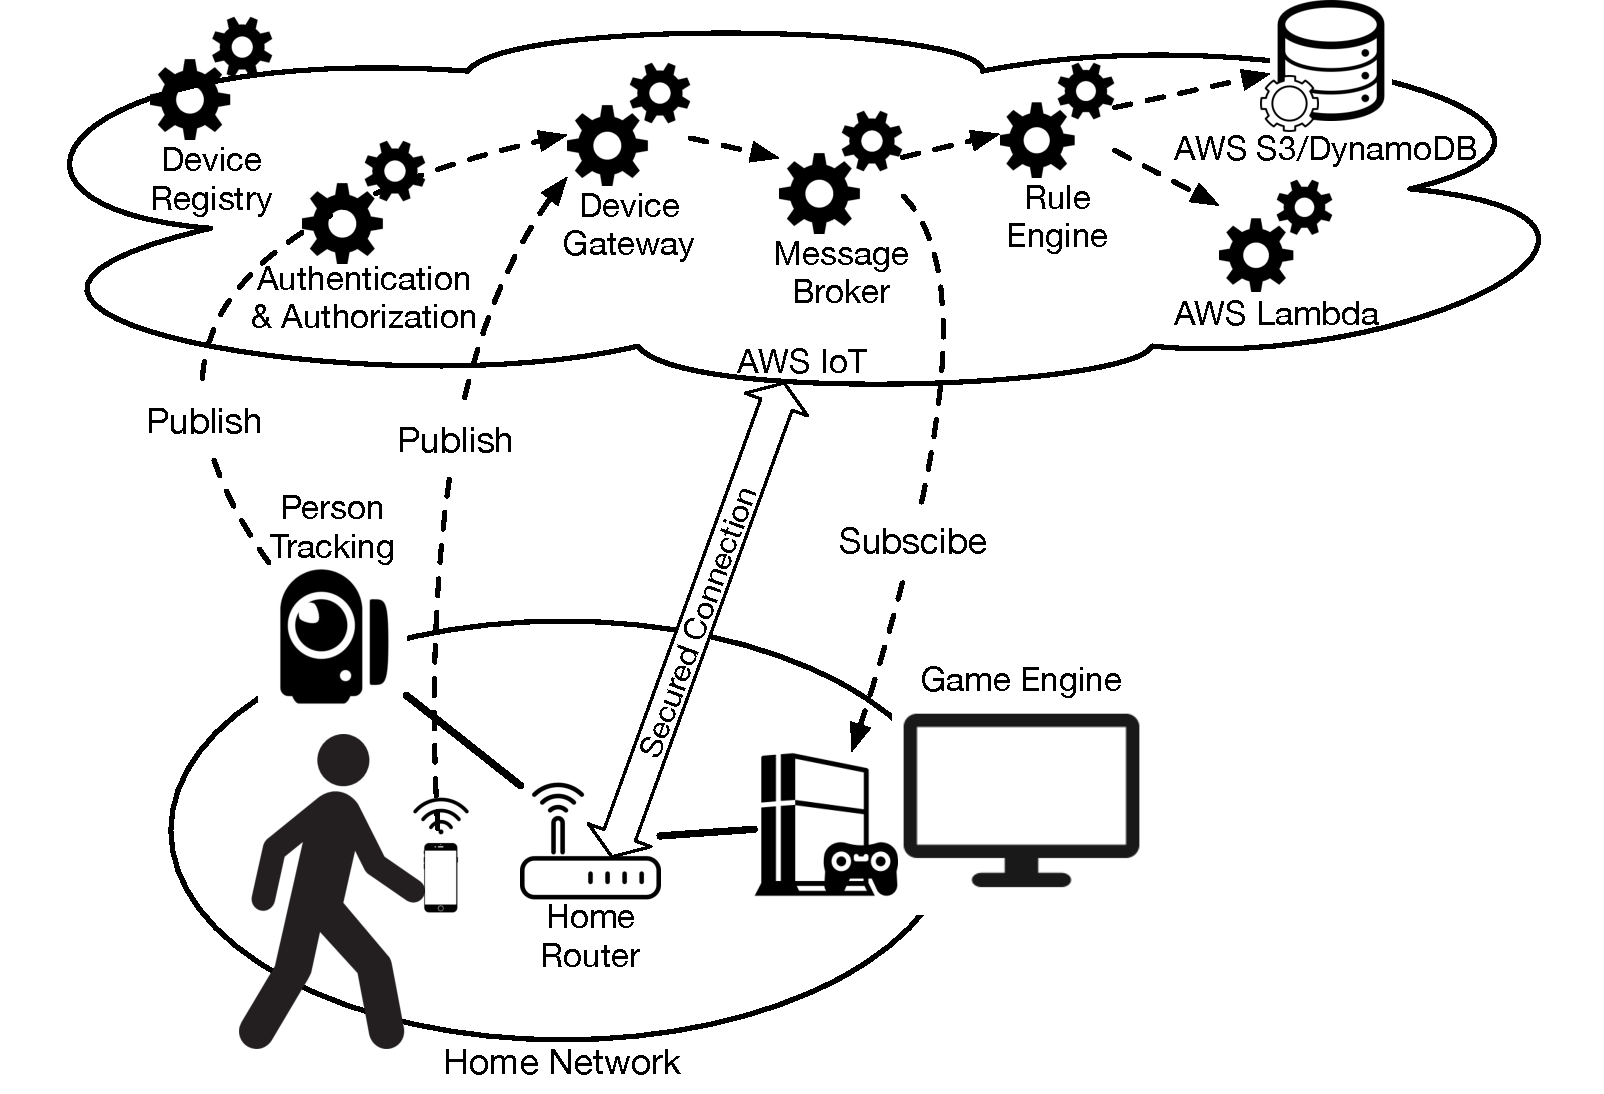
\includegraphics[width=0.37\textwidth]{aws-concept.pdf}%
\label{fig:aws-concept}}
\hfil
\subfloat[Conceptual system over HomeKit]{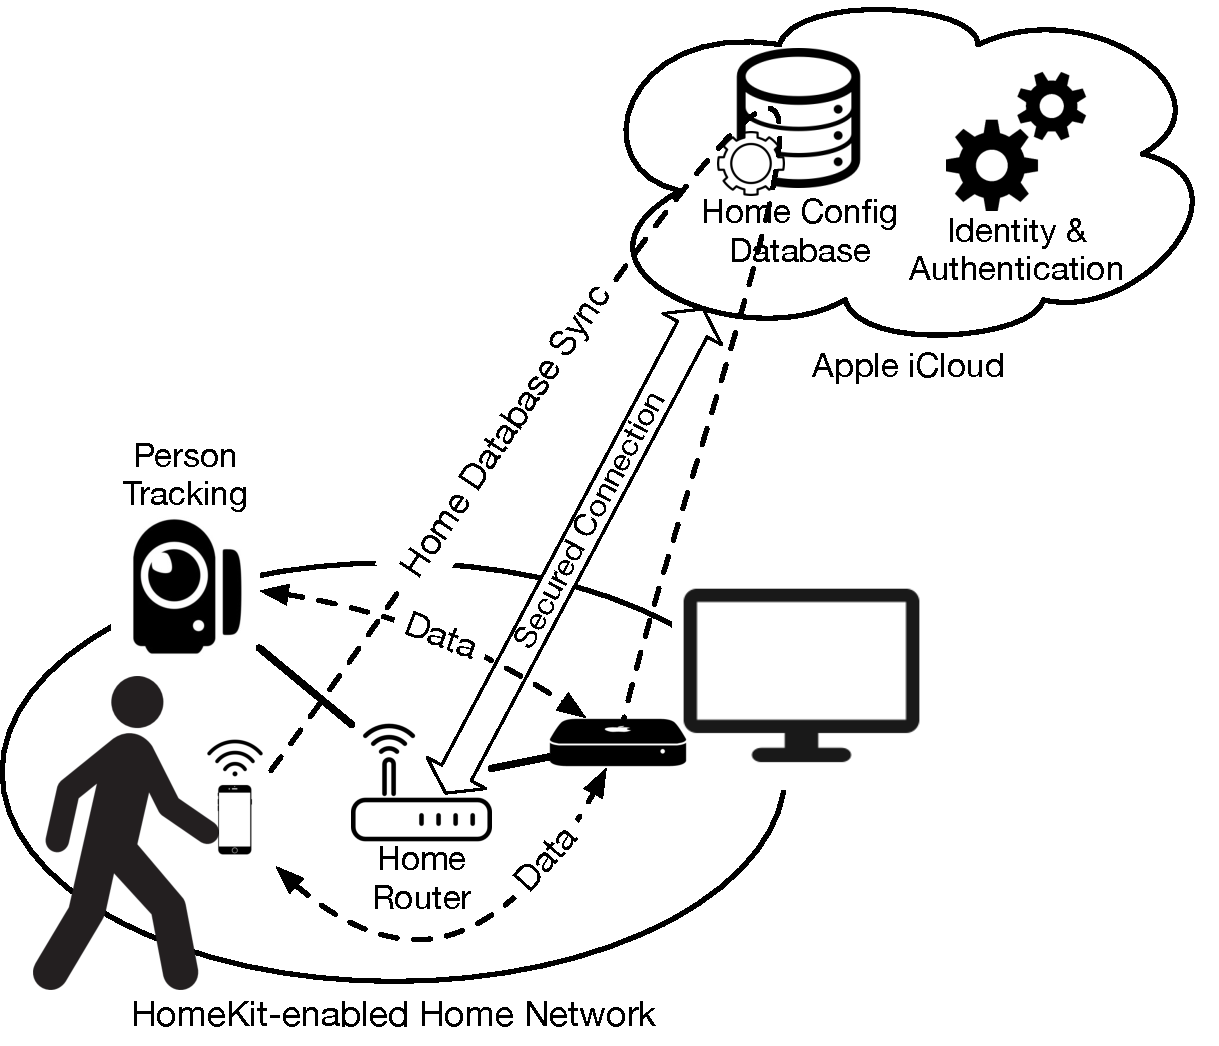
\includegraphics[width=0.3\textwidth]{homekit-concept.pdf}%
\label{fig:homekit-concept}}
\hfil
\subfloat[Actual implementation over NDN-IoT]{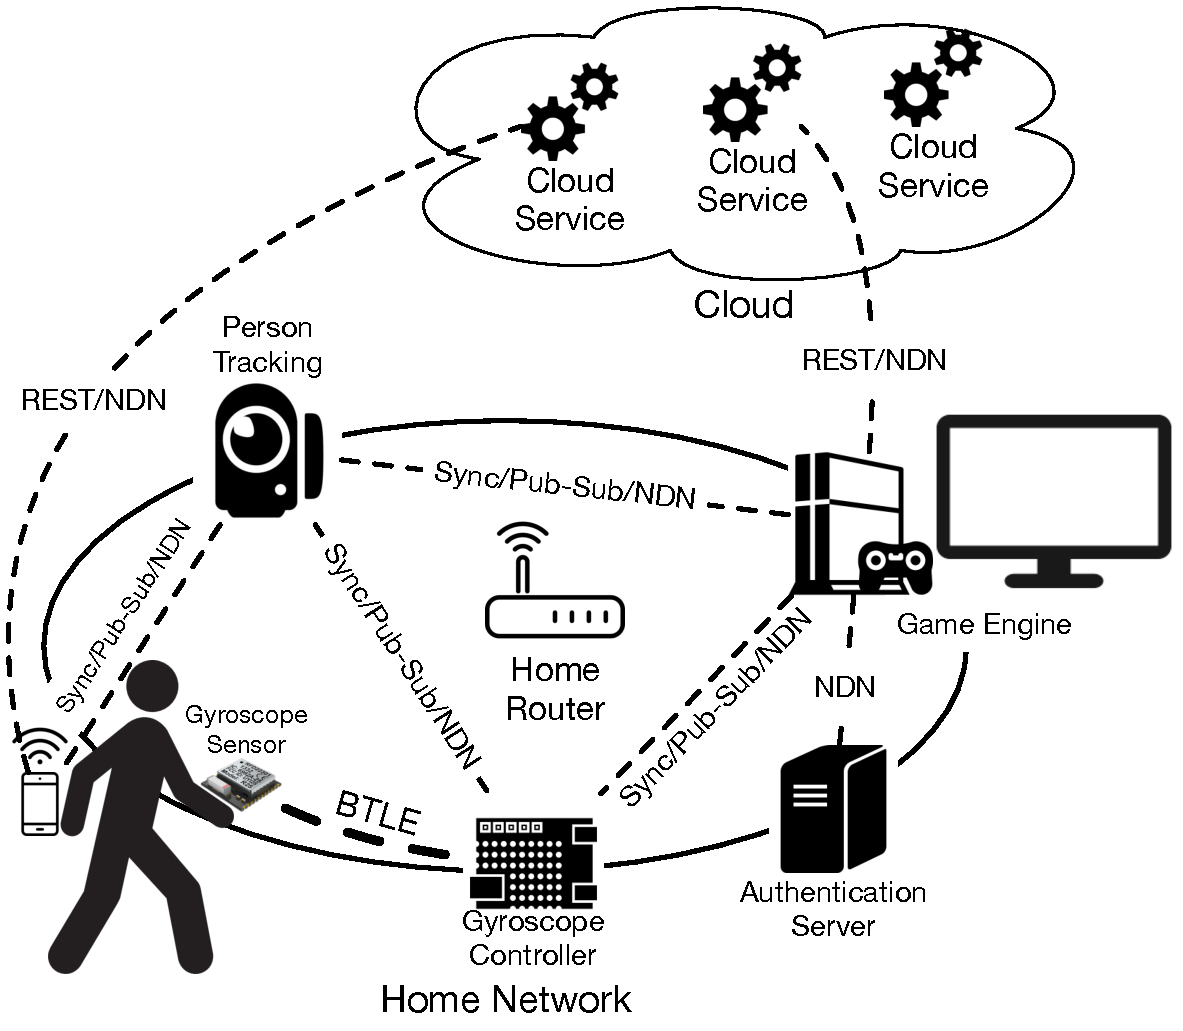
\includegraphics[width=0.3\textwidth]{flow-ndn-iot.pdf}%
\label{fig:flow-ndn-iot}}
\caption{Comparison of IoT-enabled home entertainment systems over different ecosystems.}
\label{fig:compare-ecosystems}
\end{figure*}

In Fig.~\ref{fig:aws-concept}, all local devices are certified by the AWS IoT Registry service in order to join the IoT system.
Application data generated by the person tracking device and the user smartphone need to go through the pub-sub message brokers (e.g., via MQTT) in the cloud who will route the messages to the game engine back in the local network or AWS services in the cloud according user-defined rules.
There is a significant amount of work performed by the AWS infrastructure to map user-defined device names to the underlying TLS tunnels, maintain soft-state about device configuration and latest status, manage the pub-sub channels between data producers and consumers, and enforce authentication and access control policies during message exchange.

Being the least cloud-dependent among the existing IoT ecosystems, HomeKit reduces the dependency on the cloud to two key services only:
providing and authenticating the identities of devices and users during the bootstrap phase, and synchronizing the home configuration database across multiple devices.
The game engine device in Fig.~\ref{fig:homekit-concept} can look up in its local copy of that database to discover the person tracking device and gyroscope sensor in the same local network.
There is a separate auto-configuration process based on mDNS to discover network addresses and set up direct TCP/IP connections among devices over local Wi-Fi or Ethernet.

Without requiring cloud connectivity, the NDN-IoT framework covers most of the services shown in Fig.~\ref{fig:service-arch}, with access control left as future work.\footnote{We expect to apply previous work in~\cite{nac}.}
In Flow/NDN-IoT (shown in Fig.~\ref{fig:flow-ndn-iot}), rendezvous and discovery built on top of a decentralized synchronization protocol allows the game engine to find the person tracking device and gyroscope sensors in the local network automatically;
the trust schema rooted at the local trust anchor allows the game engine to authenticate the data produced by other devices without establishing secured tunnels to either the local devices or the remote cloud;
application data messaging is efficiently supported by the NDN network layer protocol for both local and remote access, without requiring additional services to configure network addresses or resolve names to addresses;
cloud services become an optional component that facilitates, rather than dictates, the local IoT functions.


% \section{Conclusion and Future Work}
\label{sec:conclusion}

This report describes the design and implementation of Flow, an IoT home entertainment experience, and NDN-IoT framework, a set of libraries built to facilitate the development of IoT applications.

Their design showed a cloudless approach to two fundamental functions in IoT, trust management and rendezvous, both achieved by exchanging application-defined hierarchically named and secured data packets at the networking level.

We implemented the framework and application, and demonstrated a prototype in Huawei in early 2017.
% During the implementation we also expanded the functionality of NDN-CCL, and identified and fixed bugs in multiple CCL libraries.

Further tasks remain for both the framework and the application. 
Data access control should be introduced in the framework. The NDN team has proposed an encryption based access control mechanism in \cite{nbac}, which is a good starting point for experimenting inside the framework.
Discovery mechanism in the framework stands to be improved. For simplicity in implementation, current mechanism constantly does ChronoSync recovery, whose efficiency can be improved by, for example, using ChronoSync directly as one-level of indirection for name discovery.
Library interface may require more thoughts. With more applications using the framework, we can better identify what abstraction are easier for application developers, or what other general application building blocks can be added to the framework.
Finally, more efforts are required in testing the framework and application, and improving their robustness, for example, although the design conceptually supports more levels in the trust relationship, this feature is not yet tested by any application components.

% \section*{Acknowledgement}
This work is partially supported by the National Science Foundation under award CNS-1345318 and CNS-1455850, and by Futurewei Technologies. 


\bibliographystyle{IEEEtran}
\bibliography{bibliography.bib}

\end{document}

%% INSTRUCTIONS FOR FIGURES BELOW


% An example of a floating figure using the graphicx package.
% Note that \label must occur AFTER (or within) \caption.
% For figures, \caption should occur after the \includegraphics.
% Note that IEEEtran v1.7 and later has special internal code that
% is designed to preserve the operation of \label within \caption
% even when the captionsoff option is in effect. However, because
% of issues like this, it may be the safest practice to put all your
% \label just after \caption rather than within \caption{}.
%
% Reminder: the "draftcls" or "draftclsnofoot", not "draft", class
% option should be used if it is desired that the figures are to be
% displayed while in draft mode.
%
%\begin{figure}[!t]
%\centering
%\includegraphics[width=2.5in]{myfigure}
% where an .eps filename suffix will be assumed under latex, 
% and a .pdf suffix will be assumed for pdflatex; or what has been declared
% via \DeclareGraphicsExtensions.
%\caption{Simulation results for the network.}
%\label{fig_sim}
%\end{figure}

% Note that the IEEE typically puts floats only at the top, even when this
% results in a large percentage of a column being occupied by floats.


% An example of a double column floating figure using two subfigures.
% (The subfig.sty package must be loaded for this to work.)
% The subfigure \label commands are set within each subfloat command,
% and the \label for the overall figure must come after \caption.
% \hfil is used as a separator to get equal spacing.
% Watch out that the combined width of all the subfigures on a 
% line do not exceed the text width or a line break will occur.
%
%\begin{figure*}[!t]
%\centering
%\subfloat[Case I]{\includegraphics[width=2.5in]{box}%
%\label{fig_first_case}}
%\hfil
%\subfloat[Case II]{\includegraphics[width=2.5in]{box}%
%\label{fig_second_case}}
%\caption{Simulation results for the network.}
%\label{fig_sim}
%\end{figure*}
%
% Note that often IEEE papers with subfigures do not employ subfigure
% captions (using the optional argument to \subfloat[]), but instead will
% reference/describe all of them (a), (b), etc., within the main caption.
% Be aware that for subfig.sty to generate the (a), (b), etc., subfigure
% labels, the optional argument to \subfloat must be present. If a
% subcaption is not desired, just leave its contents blank,
% e.g., \subfloat[].


% An example of a floating table. Note that, for IEEE style tables, the
% \caption command should come BEFORE the table and, given that table
% captions serve much like titles, are usually capitalized except for words
% such as a, an, and, as, at, but, by, for, in, nor, of, on, or, the, to
% and up, which are usually not capitalized unless they are the first or
% last word of the caption. Table text will default to \footnotesize as
% the IEEE normally uses this smaller font for tables.
% The \label must come after \caption as always.
%
%\begin{table}[!t]
%% increase table row spacing, adjust to taste
%\renewcommand{\arraystretch}{1.3}
% if using array.sty, it might be a good idea to tweak the value of
% \extrarowheight as needed to properly center the text within the cells
%\caption{An Example of a Table}
%\label{table_example}
%\centering
%% Some packages, such as MDW tools, offer better commands for making tables
%% than the plain LaTeX2e tabular which is used here.
%\begin{tabular}{|c||c|}
%\hline
%One & Two\\
%\hline
%Three & Four\\
%\hline
%\end{tabular}
%\end{table}


% Note that the IEEE does not put floats in the very first column
% - or typically anywhere on the first page for that matter. Also,
% in-text middle ("here") positioning is typically not used, but it
% is allowed and encouraged for Computer Society conferences (but
% not Computer Society journals). Most IEEE journals/conferences use
% top floats exclusively. 
% Note that, LaTeX2e, unlike IEEE journals/conferences, places
% footnotes above bottom floats. This can be corrected via the
% \fnbelowfloat command of the stfloats package.

